%! TeX program = lualatex
% !TEX options = -outdir=build

%Use one of the two documentclass lines depending on aspect ratio needed
% for 4x3 aspect ratio slides
%\documentclass{beamer}
%for 16x9 (modern wide screen) aspect ratio slides
\documentclass[9pt,aspectratio=169,table]{beamer}
\usepackage[utf8]{inputenc}
\usepackage{csquotes}
\usepackage[
  backend=biber,
  citestyle=authoryear,
  labeldate=year
]{biblatex}
\usepackage{multicol}
\usepackage[light]{mycodestyle}
\usepackage{caption}
\usepackage{hyperref}
\usepackage{tikz}
\usepackage[spanish]{babel}
\usepackage{setspace}
\usepackage{multicol}
\usepackage{booktabs}
\usepackage{multirow}
\usepackage{colortbl}
\usepackage{dirtytalk}
\usepackage{subcaption}
\usepackage{pifont}
\usepackage{fontawesome5}
\captionsetup{font=scriptsize,labelfont=scriptsize}
\graphicspath{{img/}{./}}
\usetikzlibrary{shapes.geometric, shapes.arrows, positioning, fit, backgrounds, arrows.meta}

% Fonts ----
% Custom fonts: https://www.overleaf.com/learn/latex/Questions/I_have_a_custom_font_I%27d_like_to_load_to_my_document._How_can_I_do_this%3F#Using_custom_fonts_with_XeLaTeX_and_LuaLaTeX
\usepackage{fontspec}

\usefonttheme{serif}
\setmainfont{XCharter}
\setsansfont{Cabin}
\setmonofont{Source Code Pro}

% Bibliography
\addbibresource{bibliography.bib}
\renewcommand*{\bibfont}{\scriptsize} % Change bibliography text size
\AtEveryBibitem{\clearfield{title}}
\DefineBibliographyStrings{spanish}{
  andothers = {\textit{et al\adddot}}
}


% CCG theming
\usetheme{ccgunam}

% Set author etc info
\title[Examen de Candidatura]
{\bfseries
  % --- Spanish ---
  Estudios de Asociación Genómica
  Libres de Sesgos
  para Rasgos Complejos y Enfermedades
  en Más de 100 mil Mexicanos \\[5pt]
  \normalsize{Examen de candidatura}
}

\author[]{Ing. Roberto Olvera Hernández}
\institute[CCG - UNAM]{
  Programa de Doctorado en Ciencias Biomédicas (PDCB) \\
  Centro de Ciencias Genómicas (CCG) \\
  Universidad Nacional Autónoma de México (UNAM)
}
\date[\today]{\today} % main date for title page,

% ----- COLOR PALETTE ----
\definecolor{bluefill}{HTML}{E3F2FD}
\definecolor{bluestroke}{HTML}{2196F3}
\definecolor{grayfill}{HTML}{E0F2F1}
\definecolor{graystroke}{HTML}{009688}
\definecolor{aquafill}{HTML}{F5F5F5}
\definecolor{aquastroke}{HTML}{9E9E9E}
\definecolor{greenfill}{HTML}{E8F5E9}
\definecolor{greenstroke}{HTML}{4CAF50}
\definecolor{yellowfill}{HTML}{FFF3E0}
\definecolor{yellowstroke}{HTML}{FF9800}
\definecolor{purplefill}{HTML}{F3E5F5}
\definecolor{purplestroke}{HTML}{9C27B0}

%% Now for the actual slides %%
\begin{document}

% \nocite{*} % Prints all citations. Just for showcase, you can delete it.

\begin{frame}[plain]
  \titlepage
\end{frame}

\sffamily

% \begin{frame}{Contents}
% \begin{frame}{Orden del día}
%   \tableofcontents
% \end{frame}

% Slides
% \section{Introduction}
\section{Introducción}

% ============================================================
% Initial GWAS explanation
% ============================================================
\begin{frame}{Estudios de Asociación Genómica (GWAS)}

  \centering
  \begin{minipage}[t]{0.48\textwidth}
    \centering
    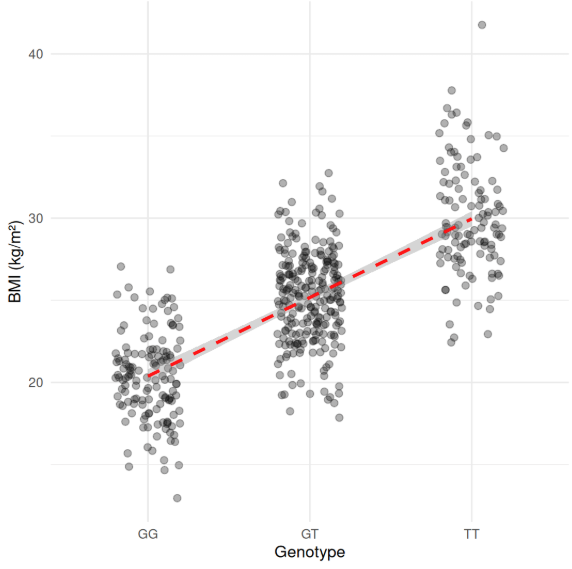
\includegraphics[width=\textwidth, height=5cm, keepaspectratio]{img/diagrams/single-locus.png}
    % \captionof{figure}{Single-variant linear model for simulated Body Mass Index (BMI) data.}
    \captionof{figure}{Modelo lineal de una sola variante con datos simulaods para Índice de Masa Corporal (BMI).}
  \end{minipage}
  \hfill
  \begin{minipage}[t]{0.48\textwidth}
    \centering
    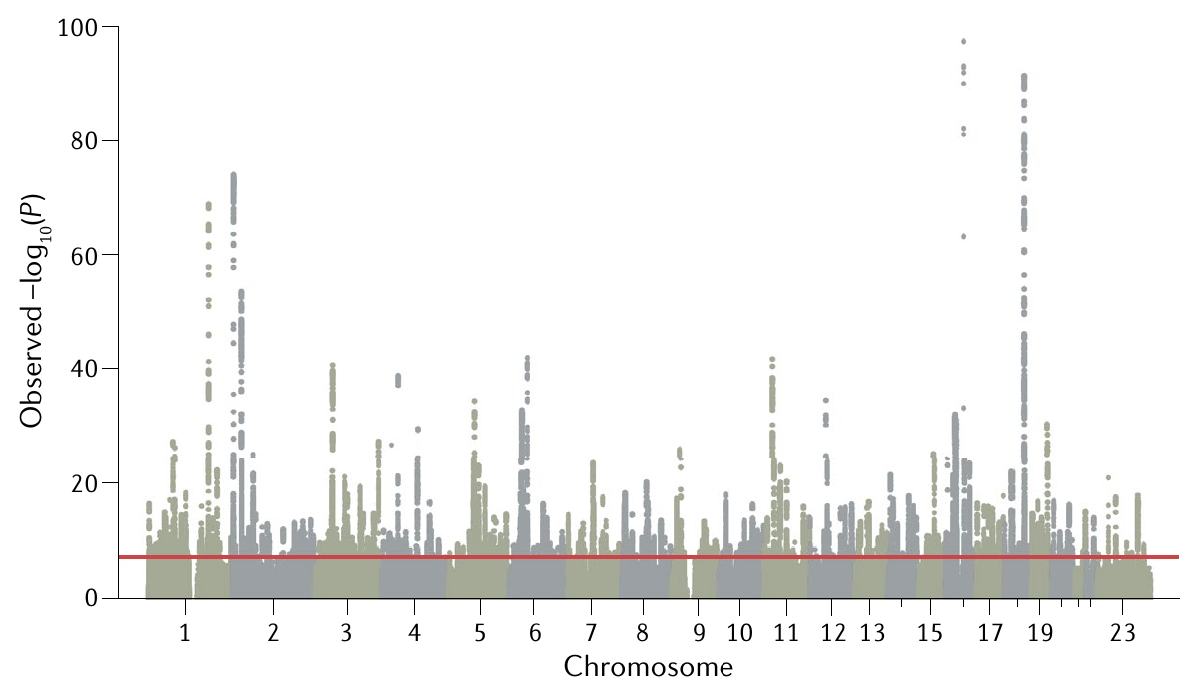
\includegraphics[width=\textwidth, height=5.5cm, keepaspectratio]{img/diagrams/manhattan.png}
    %\captionof{figure}{GWAS results showing the significance of each regression for Body Mass Index (BMI) (Uffelmann et al., 2021, Nature Methods Review).}
    \captionof{figure}{Manhattan Plot mostrando resultados de asociación de un GWAS para Índice de Masa Corporal (BMI) en una población europea. Recuperado de \parencite{uffelmann2021-gwas}.}
  \end{minipage}

\end{frame}

% ============================================================
% Animated TikZ: Genetic Effects Decomposition (two-column)
% ============================================================
\begin{frame}[b]{Sesgos en GWAS}

  \begin{columns}

    %% ---- LEFT COLUMN: stacked bar + legend ----
    \begin{column}{0.42\textwidth}
      \centering
      \begin{tikzpicture}[
        every node/.style={font=\sffamily},
      ]

        % --- Color definitions ---
        \definecolor{dgegray}{HTML}{3C3C3C}
        \definecolor{nurblue}{HTML}{1A7FA0}
        \definecolor{assred}{HTML}{7A1525}
        \definecolor{stratgray}{HTML}{B8B8B8}
        \definecolor{sideblack}{HTML}{1A1A1A}
        \definecolor{dimgray}{HTML}{D0D0D0}

        % --- Dimensions (narrower for column) ---
        \def\barW{2.4}
        \def\barX{0.7}
        \def\hdge{2.3}
        \def\hBlue{0.75}
        \def\hRed{0.6}
        \def\hGray{0.35}

        % --- Fixed bounding box (prevents bar from jumping between overlays) ---
        \useasboundingbox
          (\barX-0.8, -2.5) rectangle (\barX+\barW+0.1, \hdge+\hBlue+\hRed+\hGray+0.1);

        % --- Layer 1: dge (always visible) ---
        \fill[dgegray]
          (\barX, 0) rectangle (\barX+\barW, \hdge);

        % --- Layer 2: Crianza genética (overlay 2+) ---
        \only<2->{
          \fill[nurblue]
            (\barX, \hdge) rectangle (\barX+\barW, \hdge+\hBlue);
        }

        % --- Layer 3: Apareamiento selectivo (overlay 3+) ---
        \only<3->{
          \fill[assred]
            (\barX, \hdge+\hBlue) rectangle (\barX+\barW, \hdge+\hBlue+\hRed);
        }

        % --- Layer 4: Estratificación poblacional (overlay 4+) ---
        \only<4->{
          \fill[stratgray]
            (\barX, \hdge+\hBlue+\hRed) rectangle (\barX+\barW, \hdge+\hBlue+\hRed+\hGray);
        }

        % --- Sidebar: "Efectos de confusión" (overlay 2+) ---
        \only<2->{
          \fill[sideblack]
            (\barX-0.7, \hdge) rectangle (\barX, \hdge+\hBlue+\hRed+\hGray);
          \node[rotate=90, anchor=mid, text=white,
                font=\sffamily\bfseries\tiny]
            at (\barX-0.35, \hdge + 0.5*\hBlue + 0.5*\hRed + 0.5*\hGray)
            % {Confounding effects};
            {Efectos de confusión};
        }

        % --- Legend: order mirrors bar (top→bottom = Estrat, Apear, Crianza, dge) ---
        \def\legX{0.0}
        \def\legY{-0.5}
        \def\legSep{0.45}
        \def\legBoxW{0.25}
        \def\legBoxH{0.25}

        %% Row 0 (top): Estratificación — highlighted on overlay 4
        \only<4>{
          \fill[stratgray]
            (\legX, \legY) rectangle +(\legBoxW, -\legBoxH);
          \node[anchor=west, font=\sffamily\bfseries\scriptsize]
            at (\legX+\legBoxW+0.1, \legY-0.5*\legBoxH)
            % {Population Stratification};
            {Estratificación poblacional};
        }
        \only<1-3>{
          \fill[dimgray]
            (\legX, \legY) rectangle +(\legBoxW, -\legBoxH);
          \node[anchor=west, font=\sffamily\scriptsize, text=dimgray]
            at (\legX+\legBoxW+0.1, \legY-0.5*\legBoxH)
            % {Population Stratification};
            {Estratificación poblacional};
        }

        %% Row 1: Apareamiento selectivo — highlighted on overlay 3
        \only<3>{
          \fill[assred]
            (\legX, \legY-1*\legSep) rectangle +(\legBoxW, -\legBoxH);
          \node[anchor=west, font=\sffamily\bfseries\scriptsize, text=assred]
            at (\legX+\legBoxW+0.1, \legY-1*\legSep-0.5*\legBoxH)
            % {Assortative Mating};
            {Apareamiento selectivo};
        }
        \only<1-2,4>{
          \fill[dimgray]
            (\legX, \legY-1*\legSep) rectangle +(\legBoxW, -\legBoxH);
          \node[anchor=west, font=\sffamily\scriptsize, text=dimgray]
            at (\legX+\legBoxW+0.1, \legY-1*\legSep-0.5*\legBoxH)
            % {Assortative Mating};
            {Apareamiento selectivo};
        }

        %% Row 2: Crianza genética — highlighted on overlay 2
        \only<2>{
          \fill[nurblue]
            (\legX, \legY-2*\legSep) rectangle +(\legBoxW, -\legBoxH);
          \node[anchor=west, font=\sffamily\bfseries\scriptsize, text=nurblue]
            at (\legX+\legBoxW+0.1, \legY-2*\legSep-0.5*\legBoxH)
            % {Indirect Genetic Effects (IGEs)};
            {Efectos Genéticos Indirectos (IGEs)};
        }
        \only<1,3->{
          \fill[dimgray]
            (\legX, \legY-2*\legSep) rectangle +(\legBoxW, -\legBoxH);
          \node[anchor=west, font=\sffamily\scriptsize, text=dimgray]
            at (\legX+\legBoxW+0.1, \legY-2*\legSep-0.5*\legBoxH)
            % {Indirect Genetic Effects (IGEs)};
            {Efectos Genéticos Indirectos (IGEs)};
        }

        %% Row 3 (bottom): dge — highlighted on overlay 1
        \only<1>{
          \fill[dgegray]
            (\legX, \legY-3*\legSep) rectangle +(\legBoxW, -\legBoxH);
          \node[anchor=west, font=\sffamily\bfseries\scriptsize]
            at (\legX+\legBoxW+0.1, \legY-3*\legSep-0.5*\legBoxH)
            % {Direct Genetic Effects (DGEs)};
            {Efectos Genéticos Directos (DGEs)};
        }
        \only<2->{
          \fill[dimgray]
            (\legX, \legY-3*\legSep) rectangle +(\legBoxW, -\legBoxH);
          \node[anchor=west, font=\sffamily\scriptsize, text=dimgray]
            at (\legX+\legBoxW+0.1, \legY-3*\legSep-0.5*\legBoxH)
            % {Direct Genetic Effects (DGEs)};
            {Efectos Genéticos Directos (DGEs)};
        }

      \end{tikzpicture}
    \end{column}

    %% ---- RIGHT COLUMN: images with captions ----
    \begin{column}{0.52\textwidth}
      \centering
      \vspace{0.5cm}
      \only<1>{%
        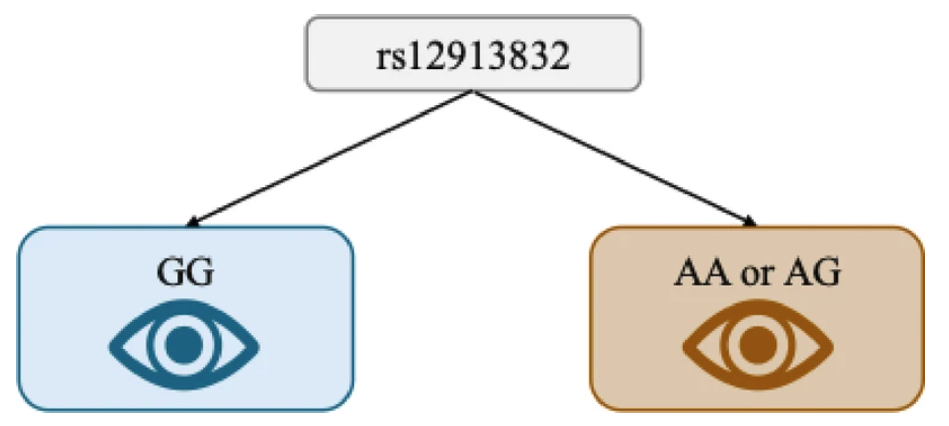
\includegraphics[width=0.95\textwidth, height=4cm, keepaspectratio]{img/diagrams/eye-color.png}%
        \captionof{figure}{Color de ojos esperado basado en el polimorfismo rs12913832 (\textit{HERC2}) en una población canadiense \parencite{abbatangelo2026-eye-color}.}%
      }%
      \only<2>{%
        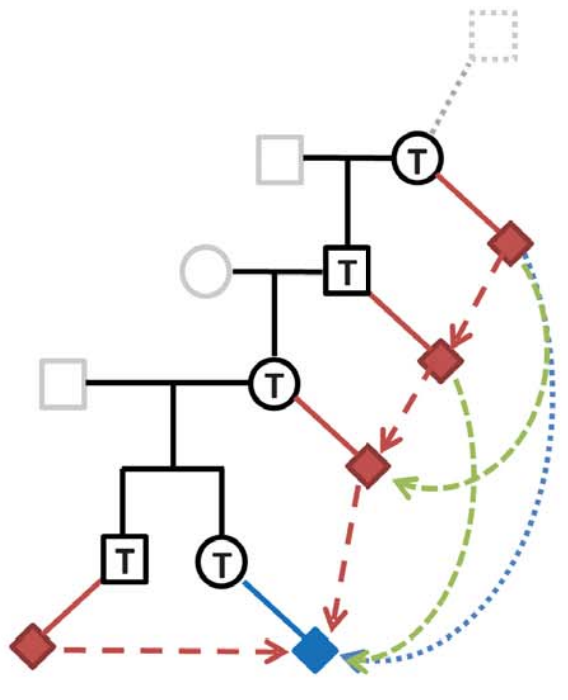
\includegraphics[width=0.95\textwidth, height=4cm, keepaspectratio]{img/diagrams/kong2018-ige.png}%
        % \captionof{figure}{Genetic nurture \parencite{kong2018-parental-genotype}.}%
        \captionof{figure}{Diagrama para el modelado de IGEs \parencite{kong2018-parental-genotype}.}%
      }%
      \only<3>{%
        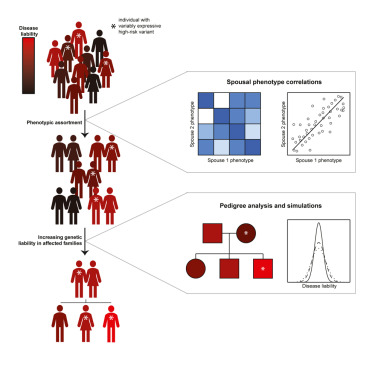
\includegraphics[width=0.95\textwidth, height=4cm, keepaspectratio]{img/diagrams/smolen2023-assortative-mating.jpg}%
        % \captionof{figure}{Assortative mating \parencite{smolen2023-assortative-mating}.}%
        \captionof{figure}{Fenotipos y genotipos (indirectamente) pueden estar correlacionados en la selección de parejas \parencite{smolen2023-assortative-mating}.}%
      }%
      \only<4>{%
        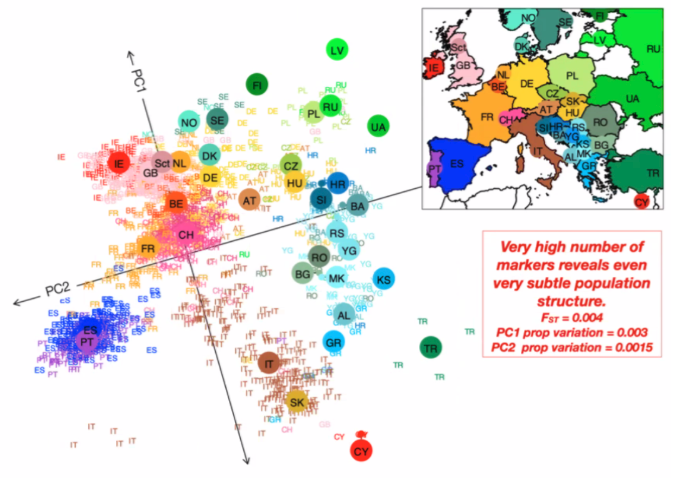
\includegraphics[width=0.95\textwidth, height=4cm, keepaspectratio]{img/diagrams/novembre2008-pca.png}%
        % \captionof{figure}{Population stratification \parencite{novembre2008-humanitiesandsocialsciences}.}%
        \captionof{figure}{Fenotipos y genotipos son segregados en regiones geográficas por barreras naturales, sociales o culturales \parencite{novembre2008-humanitiesandsocialsciences}.}%
      }%
    \end{column}
  \end{columns}
\end{frame}

% ============================================================
% Static TikZ: Genetic Effects Shrinkage
% ============================================================
\usetikzlibrary{decorations.pathreplacing, arrows.meta}

\begin{frame}{Sesgos en GWAS}
  \centering
  \vspace{0.5cm}
  \begin{tikzpicture}[
    every node/.style={font=\sffamily},
  ]

    % --- Color definitions ---
    \definecolor{dgegray}{HTML}{3C3C3C}
    \definecolor{nurblue}{HTML}{1A7FA0}
    \definecolor{assred}{HTML}{7A1525}
    \definecolor{stratgray}{HTML}{B8B8B8}
    \definecolor{sideblack}{HTML}{000000}
    \definecolor{arrowdark}{HTML}{2B3245}
    \definecolor{bracered}{HTML}{ED4E33}

    % --- Dimensions for left bar (copied from previous slide) ---
    \def\barW{2.4}
    \def\barX{-0.5}
    \def\hdge{2.3}
    \def\hBlue{0.75}
    \def\hRed{0.6}
    \def\hGray{0.35}

    % --- Dimensions for right bar ---
    \def\barXRight{6.8}
    \def\hBlueR{0.4}
    \def\hRedR{0.15}
    \def\hGrayR{0.2}

    % --- LEFT BAR ---
    % DGE
    \fill[dgegray] (\barX, 0) rectangle (\barX+\barW, \hdge);
    % Crianza / IGEs
    \fill[nurblue] (\barX, \hdge) rectangle (\barX+\barW, \hdge+\hBlue);
    % Apareamiento / Assortative
    \fill[assred] (\barX, \hdge+\hBlue) rectangle (\barX+\barW, \hdge+\hBlue+\hRed);
    % Estratificación / Pop Strat
    \fill[stratgray] (\barX, \hdge+\hBlue+\hRed) rectangle (\barX+\barW, \hdge+\hBlue+\hRed+\hGray);

    % Sidebar "Confounding effects"
    \fill[sideblack] (\barX-0.7, \hdge) rectangle (\barX, \hdge+\hBlue+\hRed+\hGray);
    \node[rotate=90, anchor=mid, text=white, font=\sffamily\bfseries\tiny]
      at (\barX-0.35, \hdge + 0.5*\hBlue + 0.5*\hRed + 0.5*\hGray)
      % {Confounding effects};
      {Efectos de confusión};

    % Left bar annotations
    \node[anchor=west, font=\sffamily\scriptsize] at (\barX+\barW+0.1, \hdge+\hBlue+\hRed+0.5*\hGray) {PCAs};
    \node[anchor=west, font=\sffamily\scriptsize] at (\barX+\barW+0.1, \hdge+\hBlue+0.5*\hRed) {LMM w/GRM};

    % --- MIDDLE ARROW ---
    \draw[-{Triangle[width=10pt,length=10pt]}, line width=5pt, color=arrowdark] 
      (\barX+\barW+2.0, \hdge+0.3) -- (\barXRight-0.5, \hdge+0.3);

    % --- RIGHT BAR ---
    % DGE (same height)
    \fill[dgegray] (\barXRight, 0) rectangle (\barXRight+\barW, \hdge);
    % IGEs (shrunk)
    \fill[nurblue] (\barXRight, \hdge) rectangle (\barXRight+\barW, \hdge+\hBlueR);
    % Assortative (shrunk)
    \fill[assred] (\barXRight, \hdge+\hBlueR) rectangle (\barXRight+\barW, \hdge+\hBlueR+\hRedR);
    % Pop Strat (shrunk)
    \fill[stratgray] (\barXRight, \hdge+\hBlueR+\hRedR) rectangle (\barXRight+\barW, \hdge+\hBlueR+\hRedR+\hGrayR);

    % Curly brace and "Inflated results"
    \draw[bracered, thick, decorate, decoration={brace, amplitude=5pt, mirror}] 
      (\barXRight+\barW+0.1, \hdge) -- (\barXRight+\barW+0.1, \hdge+\hBlueR+\hRedR+\hGrayR) 
      node[midway, right=8pt, font=\sffamily\bfseries\scriptsize, text=bracered]
      % {Inflated results};
      {Efectos poblacionales};

    % --- LEGEND (Bottom Left) ---
    \def\legX{\barX-0.7}
    \def\legY{-0.5}
    \def\legSep{0.45}
    \def\legBoxW{0.25}
    \def\legBoxH{0.25}

    % Pop Strat
    \fill[stratgray] (\legX, \legY) rectangle +(\legBoxW, -\legBoxH);
    \node[anchor=west, font=\sffamily\scriptsize] at (\legX+\legBoxW+0.1, \legY-0.5*\legBoxH)
      % {Population stratification};
      {Estratificación poblacional};

    % Assortative Mating
    \fill[assred] (\legX, \legY-1*\legSep) rectangle +(\legBoxW, -\legBoxH);
    \node[anchor=west, font=\sffamily\scriptsize] at (\legX+\legBoxW+0.1, \legY-1*\legSep-0.5*\legBoxH)
      % {Assortative mating};
      {Apareamiento selectivo};

    % IGEs
    \fill[nurblue] (\legX, \legY-2*\legSep) rectangle +(\legBoxW, -\legBoxH);
    \node[anchor=west, font=\sffamily\scriptsize] at (\legX+\legBoxW+0.1, \legY-2*\legSep-0.5*\legBoxH)
      % {Indirect Genetic Effects (IGEs)};
      {Efectos Genéticos Indirectos (IGEs)};

    % DGEs
    \fill[dgegray] (\legX, \legY-3*\legSep) rectangle +(\legBoxW, -\legBoxH);
    \node[anchor=west, font=\sffamily\bfseries\scriptsize] at (\legX+\legBoxW+0.1, \legY-3*\legSep-0.5*\legBoxH)
      % {Direct Genetic Efects (DGEs)};
      {Efectos Genéticos Directos (DGEs)};

    % --- CITATION (Bottom Right) ---
    \node[anchor=south east, font=\sffamily\scriptsize] 
      at (\barXRight+\barW+2.5, \legY-3*\legSep-0.5*\legBoxH) 
      % {Adapted from \textcite{young2019-genetic-effects}.};
      {Diagrama adptado de \textcite{young2019-genetic-effects}.};

  \end{tikzpicture}
\end{frame}

% ============================================================
% Family-based GWAS Limitations
% ============================================================
\begin{frame}[c]{Family-based GWAS}
  \begin{columns}[c]

    % --- LEFT COLUMN: Image ---
    \begin{column}{0.55\textwidth}
      \centering
      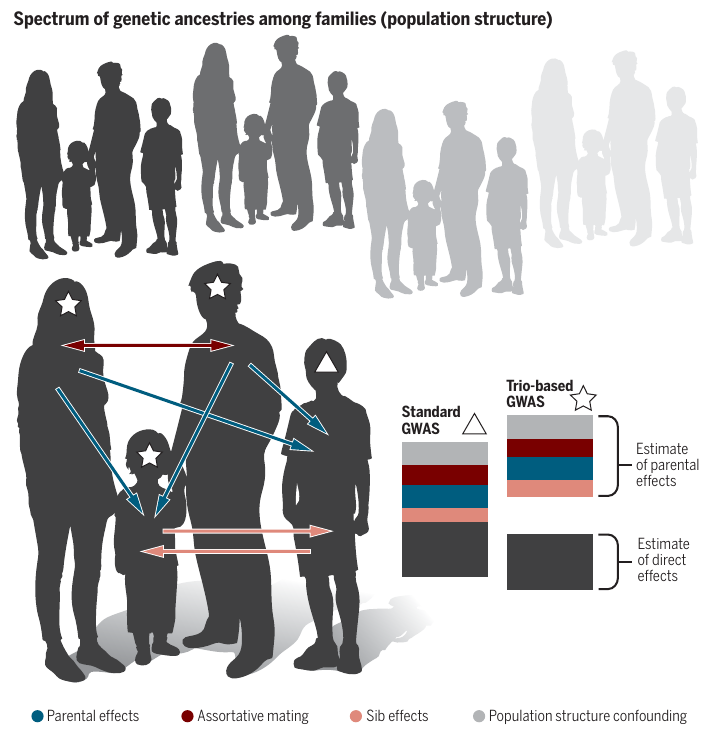
\includegraphics[height=5.15cm, keepaspectratio]{img/diagrams/young2019-signals-captured-gwas.png}
      % \captionof{figure}{Signals captured by GWAS of related individuals and families \parencite{young2019-genetic-effects}.}
      \captionof{figure}{Señales capturadas por un GWAS de individuos relacionados y familias. Recuperado de \textcite{young2019-genetic-effects}.}
    \end{column}

    % --- RIGHT COLUMN: Text ---
    \begin{column}{0.45\textwidth}

      % --- Spanish ---
      {Los FGWAS pueden discriminar entre DGEs y Efectos Poblacionales} \\[1pt]
      {\tiny \parencite{visscher2006-populationgenetics,young2019-genetic-effects}}\\[1em]
      \pause
      \centering
      {\bfseries\large\color[HTML]{7CBB00}
        PERO
      }\\[0.5em]
      \begin{columns}[T]
        \small
        \begin{column}{0.425\textwidth}
          {Evidencia de una señal biológica \textbf{verdadera}}
        \end{column}
        \begin{column}{0.05\textwidth}
          vs.
        \end{column}
        \begin{column}{0.425\textwidth}
          {Limitado a solamente individuos con \textbf{ambos padres genotipados}}
        \end{column}
      \end{columns}
      \pause
      \vspace{3em}
      {\centering\large
        Recuperar poder estadístico es \textbf{prioridad}
      }
    \end{column}
  \end{columns}
\end{frame}

% ============================================================
% Why use the MCPS?
% ============================================================
 \begin{frame}[c]{Estudio Prospectivo de la Ciudad de México (MCPS)}
  \begin{columns}[T]
    % --- COLUMN A ---
    \begin{column}{0.35\textwidth}
      \centering
      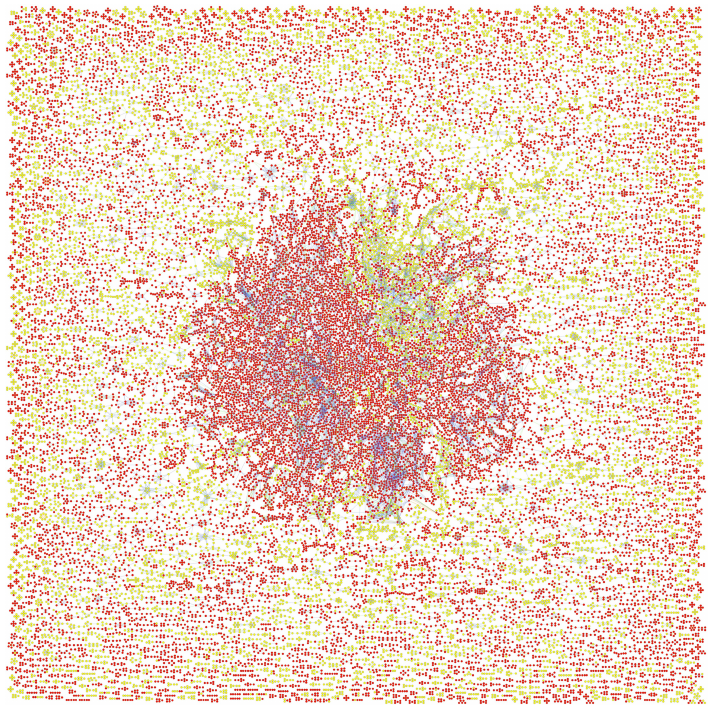
\includegraphics[height=3cm]{img/diagrams/mcps-family-network.png}\\[0.5em]
      {\bfseries
        Redes familiares densas
      }\\[3pt]
      {\tiny
        MCPS \parencite{ziyatdinov2023-mcps} proporciona más del \textit{doble} de pares de familiares de primer grado que UK Biobank \parencite{bycroft2018-ukbiobank} \\[2pt]
      }
    \end{column}
    % --- COLUMN B ---
    \begin{column}{0.65\textwidth}
      \centering
      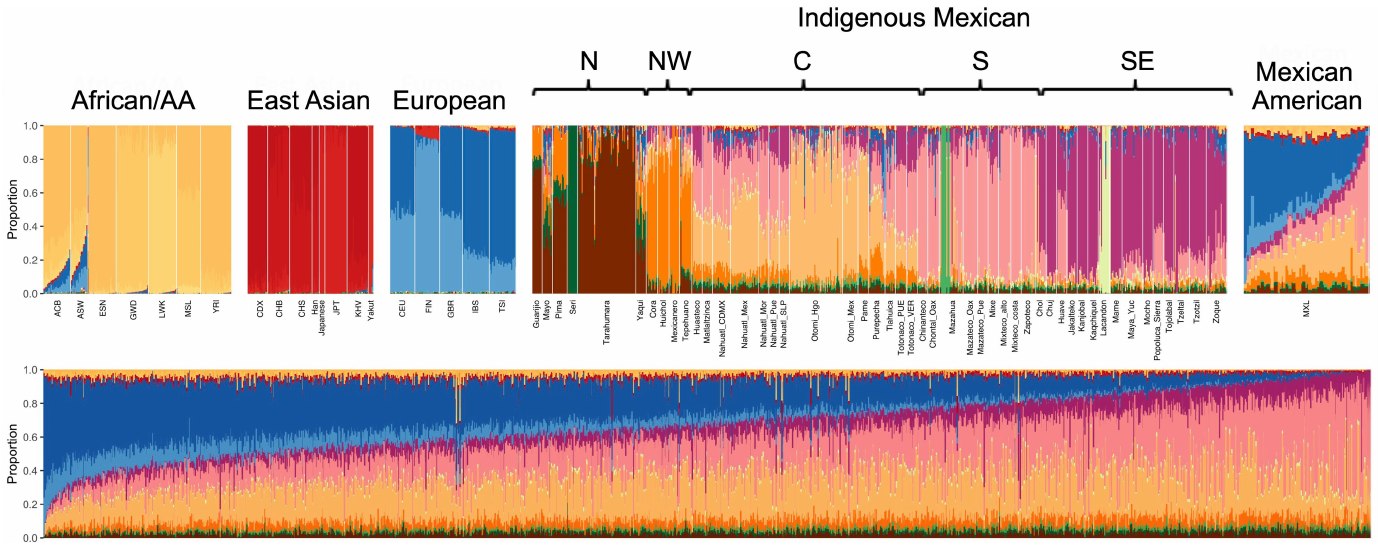
\includegraphics[height=3cm]{img/diagrams/mcps-admixture.png}\\[0.5em]
      {\bfseries
        Mestizaje reciente
      }\\[3pt]
      {\tiny
        Ancestrías provenientes de Europa y África, e indígenas de México.
        Mejorar representación en estudios genómicos \parencite{popejoy2016-admixture,martin2017-pgs}.
      }
    \end{column}
  \end{columns}
  \centering
  \vspace{2em}
  {\small
    \textcite{tapia-conyer2006-mcps,ziyatdinov2023-mcps}
  }
\end{frame}
% ponytail: YAGNI! No macros with `#` inside a beamer frame to avoid fragile errors.

\begin{frame}[t]{Metodolgía: Resumen visual}
    \centering
    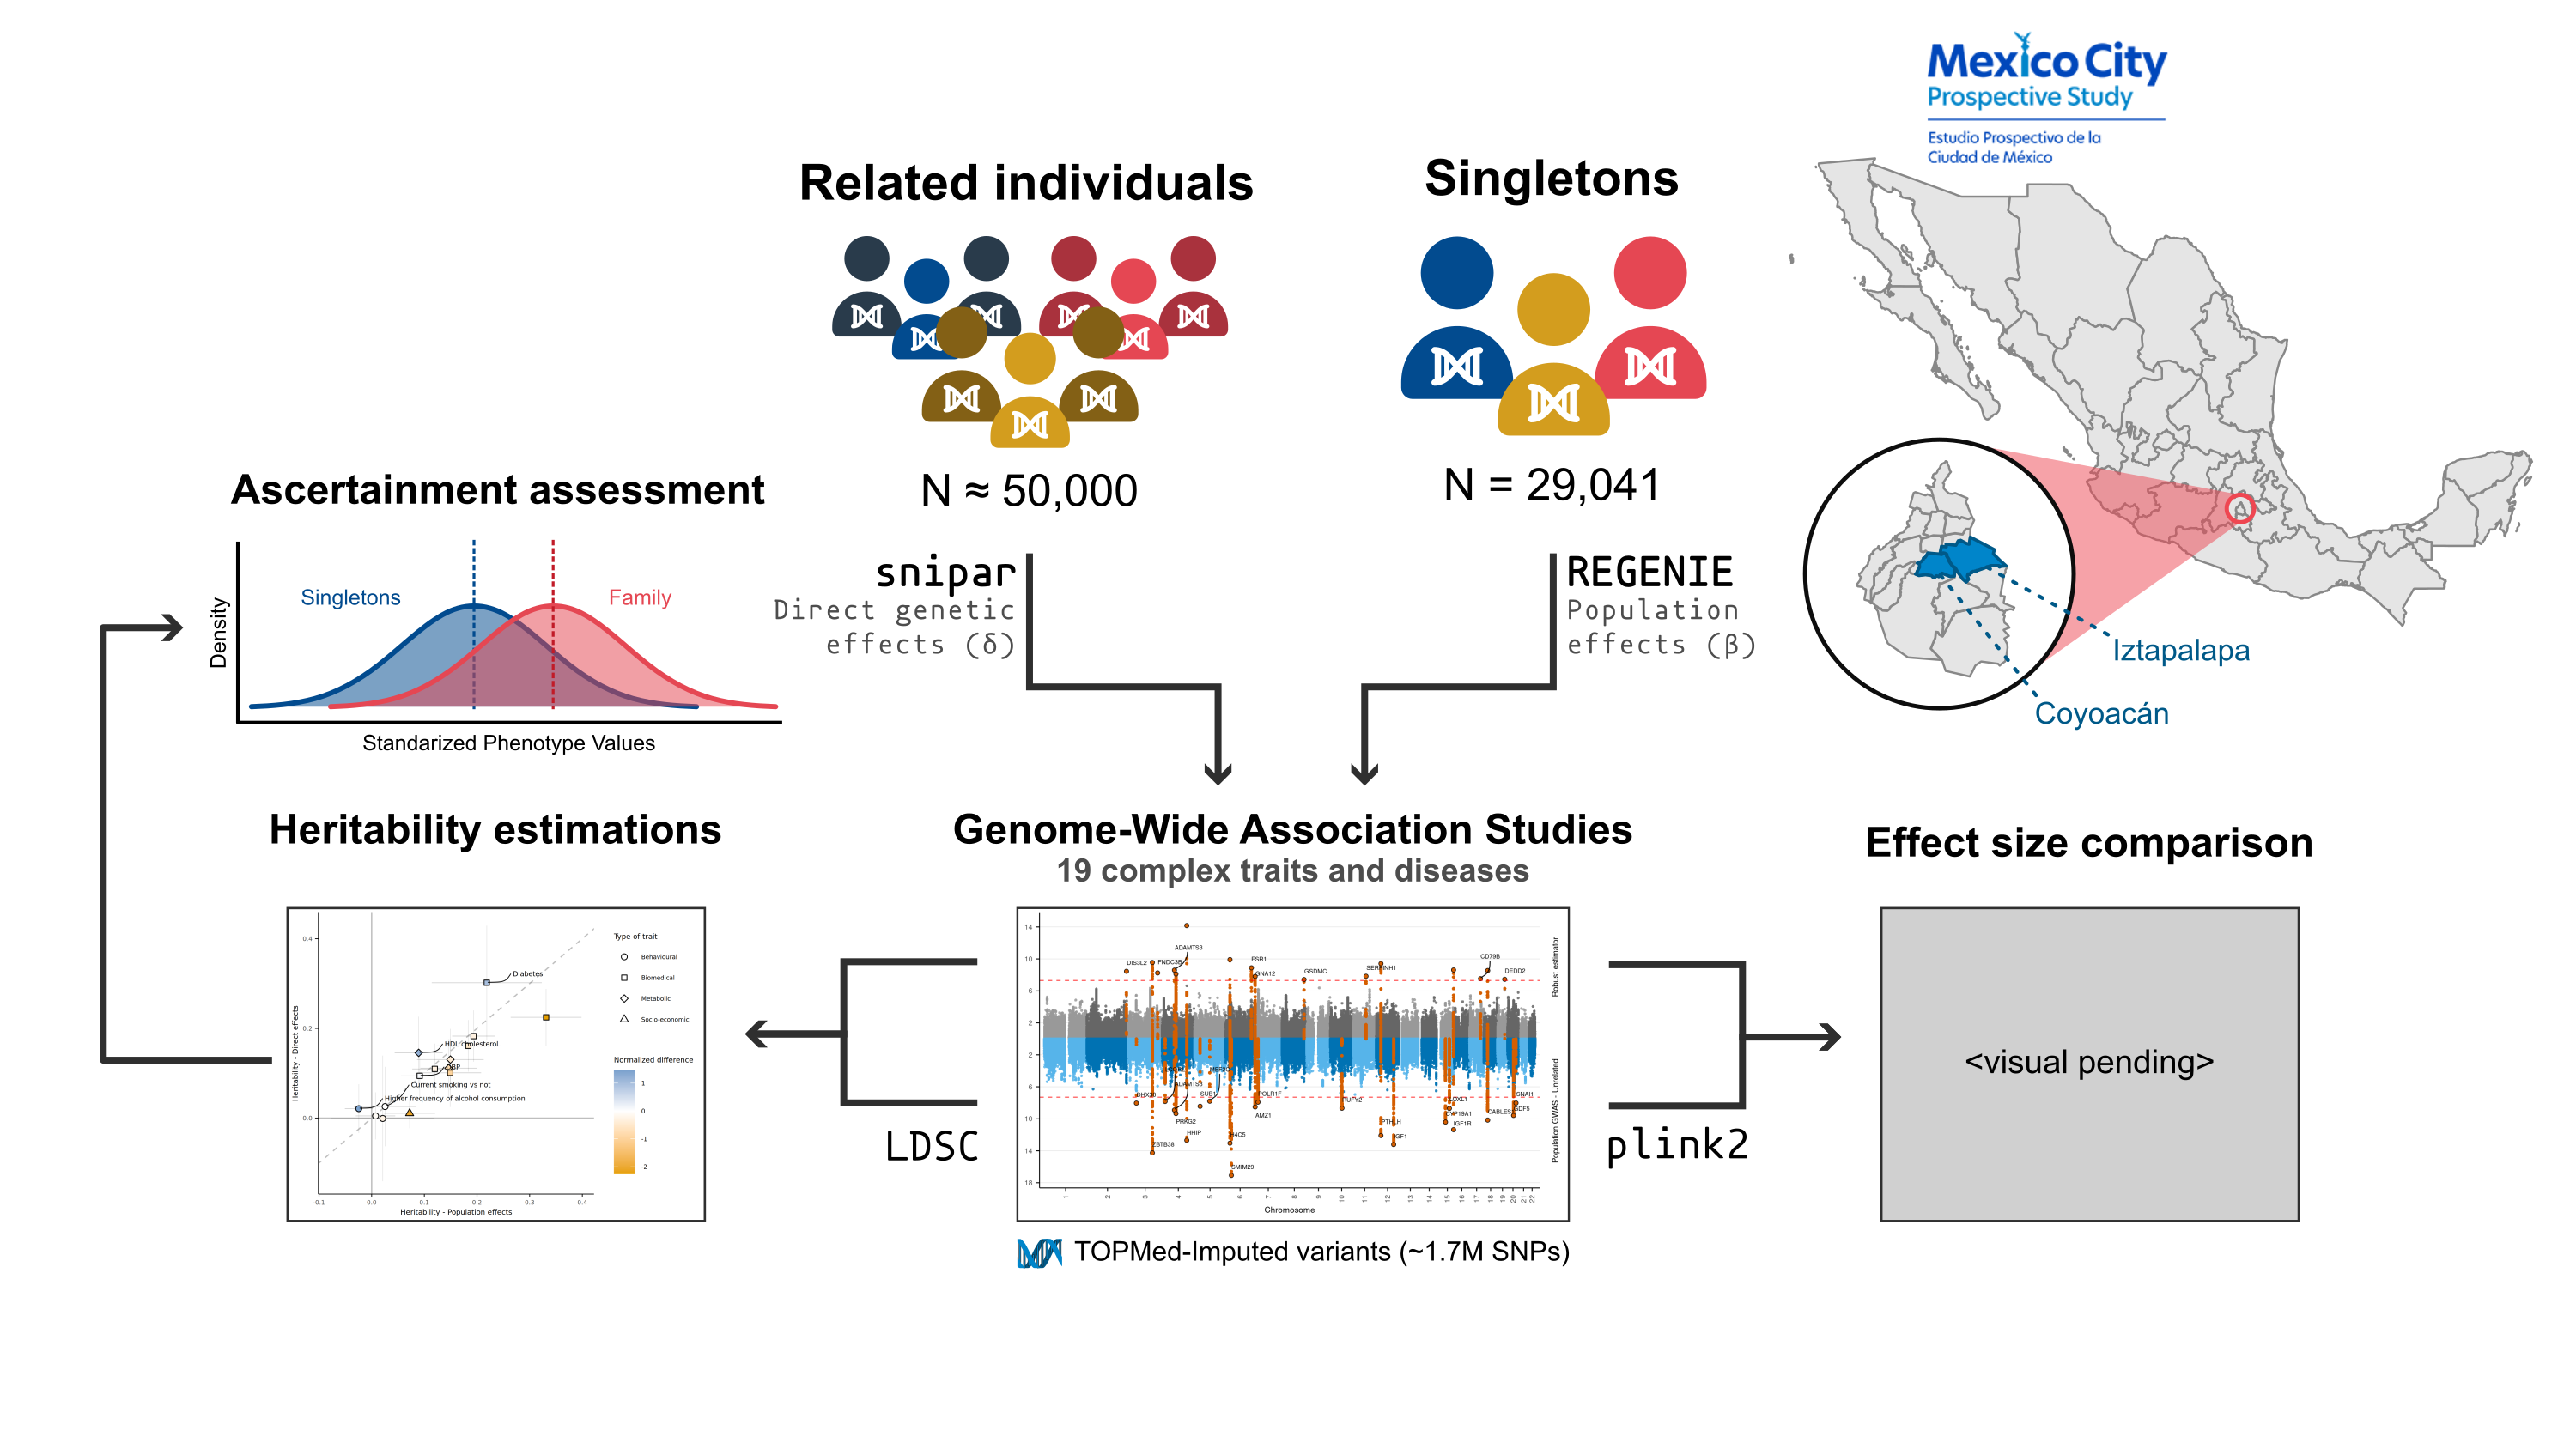
\includegraphics[height=\textheight]{img/diagrams/visual-abstract.png}
\end{frame}

% ---- Option C: Cascading Incremental ----
% ponytail: plain TikZ, no # args, hardcoded positions
\begin{frame}[b]{Diseño experimental: Escalamiento incremental}
\resizebox{!}{0.85\textheight}{
\centering
\begin{tikzpicture}

% ---- Column geometry (widening per semester) ----
% Labels
\def\lw{3.0}
% S1: x=3.15, w=1.5
% S2: x=4.85, w=2.2
% S3: x=7.25, w=3.0
% S4: x=10.45, w=3.4

% ---- Row y positions ----
% headers: 0.4
% scope: -0.15
% separator: -0.55
% IBD: -1.0
% Imp: -1.65
% FGWAS: -2.3
% LDSC: -2.95
% PRS: -3.6

\def\barH{0.45}

% ==== SEMESTER HEADERS ====
\node[fill=ccgblue, text=white, font=\footnotesize\bfseries, rounded corners=2pt, minimum width=2.45cm, minimum height=0.45cm] at (4.375, 0.4) {S1};
\node[fill=unamgold, text=white, font=\footnotesize\bfseries, rounded corners=2pt, minimum width=2.45cm, minimum height=0.45cm] at (7.125, 0.4) {S2};
\node[fill=green, text=white, font=\footnotesize\bfseries, rounded corners=2pt, minimum width=2.45cm, minimum height=0.45cm] at (9.875, 0.4) {S3};
\node[fill=red, text=white, font=\footnotesize\bfseries, rounded corners=2pt, minimum width=2.45cm, minimum height=0.45cm] at (12.625, 0.4) {S4};

% ==== SCOPE: 3-row icon grid ====
% Row 1: Database (\faDatabase)
\node[font=\footnotesize, text=black!50, anchor=east] at (2.9, -0.1) {\faDatabase};
\node[font=\scriptsize, text=ccgblue] at (4.375, -0.1)  {GSAv2 CHIP};
\node[font=\scriptsize, text=unamgold] at (7.125, -0.1) {TOPMed Imputed};
\node[font=\scriptsize, text=green] at (9.875, -0.1)    {TOPMed Imputed};
\node[font=\scriptsize, text=red] at (12.625, -0.1)     {TOPMed Imputed};

% Row 2: Chromosomes (\faDna)
\node[font=\footnotesize, text=black!50, anchor=east] at (2.9, -0.4) {\faDna};
\node[font=\scriptsize, text=ccgblue] at (4.375, -0.4)  {Chr. 22};
\node[font=\scriptsize, text=unamgold] at (7.125, -0.4) {Chr. 1--22};
\node[font=\scriptsize, text=green] at (9.875, -0.4)    {Chr. 1--22};
\node[font=\scriptsize, text=red] at (12.625, -0.4)     {Chr. 1--22};

% Row 3: Traits (\faHeartbeat)
\node[font=\scriptsize, text=black!50, anchor=east] at (2.9, -0.7) {\faHeartbeat};
\node[font=\scriptsize, text=ccgblue] at (4.375, -0.7) {3 rasgos};
\node[font=\scriptsize, text=unamgold] at (7.125, -0.7) {13 rasgos};
\node[font=\scriptsize, text=green] at (9.875, -0.7) {17 rasgos};
\node[font=\scriptsize, text=red] at (12.625, -0.7) {28 rasgos};

% ==== SEPARATOR LINE ====
\draw[gray!40, thin] (0, -1.0) -- (13.85, -1.0);

% ==== ROW LABELS ====
\node[font=\scriptsize, anchor=east] at (2.9, -1.4) {IBD entre hermanos};
\node[font=\scriptsize, anchor=east] at (2.9, -2.0) {Imputación Mendeliana};
\node[font=\scriptsize, anchor=east] at (2.9, -2.6) {GWAS (REGENIE)};
\node[font=\scriptsize, anchor=east] at (2.9, -3.2) {FGWAS (\textit{Sibpair/Trios})};
\node[font=\scriptsize, anchor=east] at (2.9, -3.8) {FGWAS (\textit{Imputed})};
\node[font=\scriptsize, anchor=east] at (2.9, -4.4) {FGWAS (\textit{Robust estimator})};
\node[font=\scriptsize, anchor=east] at (2.9, -5.0) {Correlaciones genéticas \& Heredabilidad};
\node[font=\scriptsize, anchor=east] at (2.9, -5.6) {Fine-mapping};

% ==== BARS ====
% --- IBD ---
\draw[gray!20, dashed, rounded corners=2pt] (3.15, {-1.4-\barH/2}) rectangle (5.6, {-1.4+\barH/2});
\fill[unamgold!70, rounded corners=2pt] (5.9, {-1.4-\barH/2}) rectangle (8.35, {-1.4+\barH/2});
\node[font=\tiny, text=black!40] at (9.875, -1.4) {\faCheck};
\node[font=\tiny, text=black!40] at (12.625, -1.4) {\faCheck};

% --- Imputación ---
\draw[gray!20, dashed, rounded corners=2pt] (3.15, {-2.0-\barH/2}) rectangle (5.6, {-2.0+\barH/2});
\fill[unamgold!70, rounded corners=2pt] (5.9, {-2.0-\barH/2}) rectangle (8.35, {-2.0+\barH/2});
\node[font=\tiny, text=black!40] at (9.875, -2.0) {\faCheck};
\node[font=\tiny, text=black!40] at (12.625, -2.0) {\faCheck};

% --- GWAS ---
\draw[gray!20, dashed, rounded corners=2pt] (3.15, {-2.6-\barH/2}) rectangle (5.6, {-2.6+\barH/2});
\draw[gray!20, dashed, rounded corners=2pt] (5.9, {-2.6-\barH/2}) rectangle (8.35, {-2.6+\barH/2});
\fill[green!70, rounded corners=2pt] (8.65, {-2.6-\barH/2}) rectangle (11.1, {-2.6+\barH/2});
\fill[red!70, rounded corners=2pt] (11.4, {-2.6-\barH/2}) rectangle (13.85, {-2.6+\barH/2});

% --- FGWAS (est. 1): S1 only ---
\fill[ccgblue!50, rounded corners=2pt] (3.15, {-3.2-\barH/2}) rectangle (5.6, {-3.2+\barH/2});
\draw[gray!20, dashed, rounded corners=2pt] (5.9, {-3.2-\barH/2}) rectangle (8.35, {-3.2+\barH/2});
\draw[gray!20, dashed, rounded corners=2pt] (8.65, {-3.2-\barH/2}) rectangle (11.1, {-3.2+\barH/2});
\draw[gray!20, dashed, rounded corners=2pt] (11.4, {-3.2-\barH/2}) rectangle (13.85, {-3.2+\barH/2});

% --- FGWAS (est. 2): S1, S2 ---
\fill[ccgblue!50, rounded corners=2pt] (3.15, {-3.8-\barH/2}) rectangle (5.6, {-3.8+\barH/2});
\fill[unamgold!70, rounded corners=2pt] (5.9, {-3.8-\barH/2}) rectangle (8.35, {-3.8+\barH/2});
\draw[gray!20, dashed, rounded corners=2pt] (8.65, {-3.8-\barH/2}) rectangle (11.1, {-3.8+\barH/2});
\draw[gray!20, dashed, rounded corners=2pt] (11.4, {-3.8-\barH/2}) rectangle (13.85, {-3.8+\barH/2});

% --- FGWAS (est. 3): S3, S4 ---
\draw[gray!20, dashed, rounded corners=2pt] (3.15, {-4.4-\barH/2}) rectangle (5.6, {-4.4+\barH/2});
\draw[gray!20, dashed, rounded corners=2pt] (5.9, {-4.4-\barH/2}) rectangle (8.35, {-4.4+\barH/2});
\fill[green!70, rounded corners=2pt] (8.65, {-4.4-\barH/2}) rectangle (11.1, {-4.4+\barH/2});
\fill[red!70, rounded corners=2pt] (11.4, {-4.4-\barH/2}) rectangle (13.85, {-4.4+\barH/2});

% --- Correlaciones genéticas & Heredabilidad ---
\draw[gray!20, dashed, rounded corners=2pt] (3.15, {-5.0-\barH/2}) rectangle (5.6, {-5.0+\barH/2});
\fill[unamgold!70, rounded corners=2pt] (5.9, {-5.0-\barH/2}) rectangle (8.35, {-5.0+\barH/2});
\fill[green!70, rounded corners=2pt] (8.65, {-5.0-\barH/2}) rectangle (11.1, {-5.0+\barH/2});
\fill[red!70, rounded corners=2pt] (11.4, {-5.0-\barH/2}) rectangle (13.85, {-5.0+\barH/2});

% --- Fine-mapping: S4 only ---
\draw[gray!20, dashed, rounded corners=2pt] (3.15, {-5.6-\barH/2}) rectangle (5.6, {-5.6+\barH/2});
\draw[gray!20, dashed, rounded corners=2pt] (5.9, {-5.6-\barH/2}) rectangle (8.35, {-5.6+\barH/2});
\draw[gray!20, dashed, rounded corners=2pt] (8.65, {-5.6-\barH/2}) rectangle (11.1, {-5.6+\barH/2});
\fill[red!70, rounded corners=2pt] (11.4, {-5.6-\barH/2}) rectangle (13.85, {-5.6+\barH/2});

% ==== BOTTOM ARROW showing progression ====
\draw[-{Stealth[length=3mm]}, thick, gray!50] (3.15, -6.3) -- (13.85, -6.3);
\node[font=\footnotesize, text=gray!60, anchor=north] at (8.5, -6.35) {Alcance incremental};

\end{tikzpicture}
}
\end{frame}
% \section{Results}
\section{Resultados}

% --- EFFECTIVE SAMPLE SIZE ---
\begin{frame}[c]{Tamaños Efectivos de Muestra}
  \begin{columns}[b]
    % --- LEFT COLUMN ----
    \begin{column}{0.64\textwidth}
      \centering
      
\includegraphics[width=\linewidth]{img/results/2026-02/effective-sample-sizes_robust-estimator_sibpair-trios.png}
    \end{column}
    % --- RIGHT COLUMN ----
    \begin{column}{0.36\textwidth}
      % --- UPPER QUADRANT ----
      \small\sffamily

      El estimador robusto tiene un mayor poder estadístico
      que el modelo de \textcite{young2022-fgwas}

      % --- LOWER QUADRANT ----
      \vspace{1cm}
      \vfill
      \captionof{figure}{
        \textbf{Comparación de tamaños efectivos de muestra para todos los rasgos en dos estimadores de FGWAS.}
        El estimador robusto vs. de pares de hermanos y trios parentales,
        incremento de 36.58\% (SD $\pm$ 6.78\%).
        Barras de error representan intervalos de confianza del 95\%.
      }
    \end{column}
  \end{columns}
\end{frame}

% --- HERITABILITY ---
\begin{frame}[c]{Comparación entre estimaciones de heredabilidad}
\begin{figure}
    \begin{minipage}[b]{0.67\textwidth}
        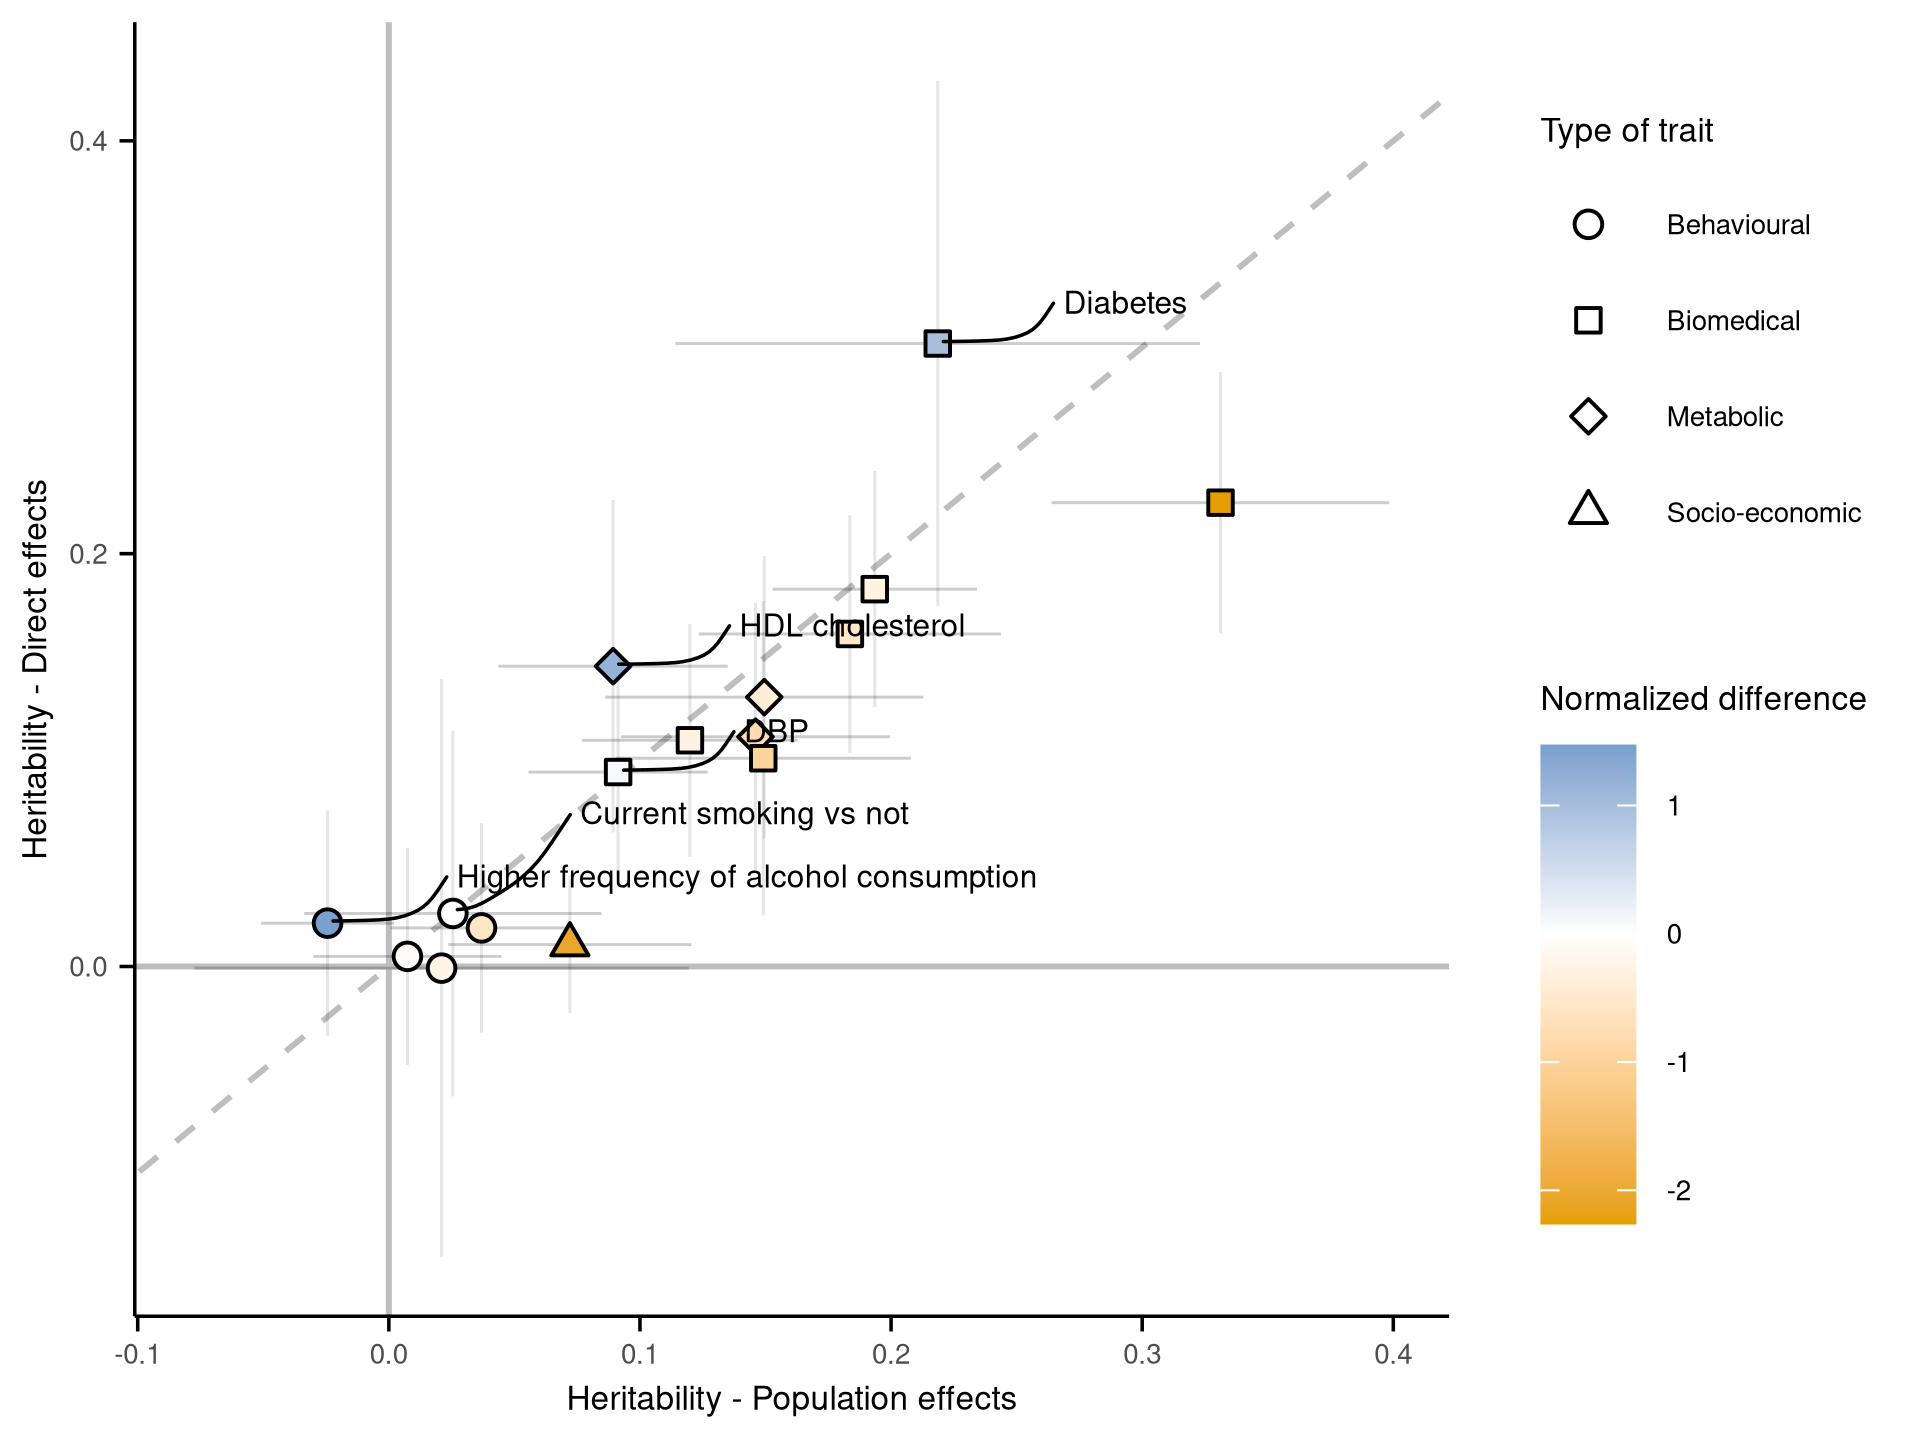
\includegraphics[width=0.95\textwidth]{img/results/2027-01/heritability/heritability_comparison.scatter.png}
    \end{minipage}\hfill
    \begin{minipage}[b]{0.33\textwidth}
        \caption{
            \textbf{Comparación de estimaciones de heredabilidad derivadas de FGWAS contra PopGWAS.}
            Cada punto representa un rasgo complejo.
            Los colores representan la clasificación.
            La línea punteada representa la línea de identidad.
            Barras de error representan intervalos de confianza al 95\%.
        }
    \end{minipage}
\end{figure}
\end{frame}

\begin{frame}[b]{Comparación de prevalencias entre subcohortes}
  \begin{figure}[htpb]
      \centering
      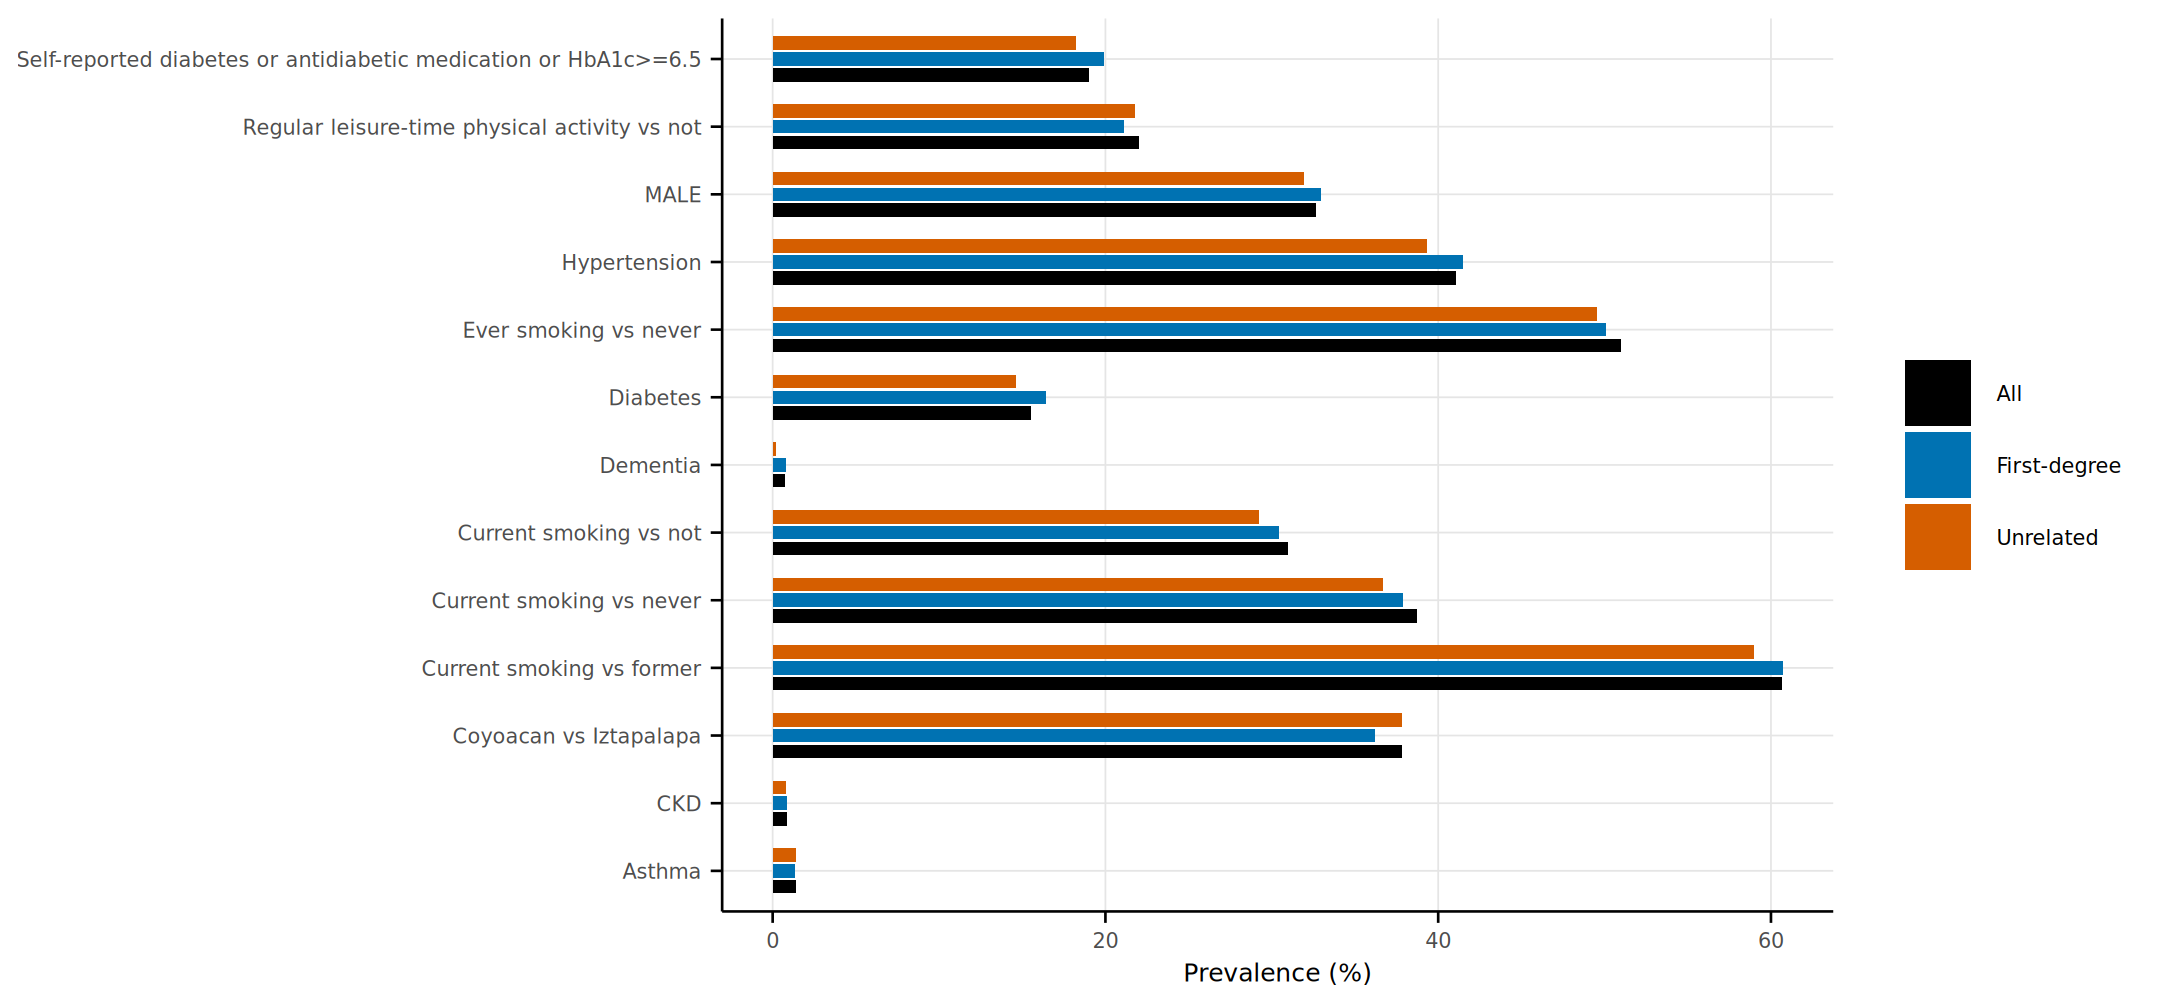
\includegraphics[width=0.9\textwidth, height=0.75\textheight, keepaspectratio]{img/results/2027-01/phenotype-smd-analyses/prevalence_comparison.cropped.png}
      \caption{
        \textbf{Comparación de prevalencias.} Prevalencias de fenotipos por subcohorte. \parencite{young2022-fgwas}
      }
      \label{fig:prevalences}
  \end{figure}
\end{frame}

\begin{frame}[c]{Comparación entre estimaciones de heredabilidad}
  \begin{figure}[htpb]
      \centering
      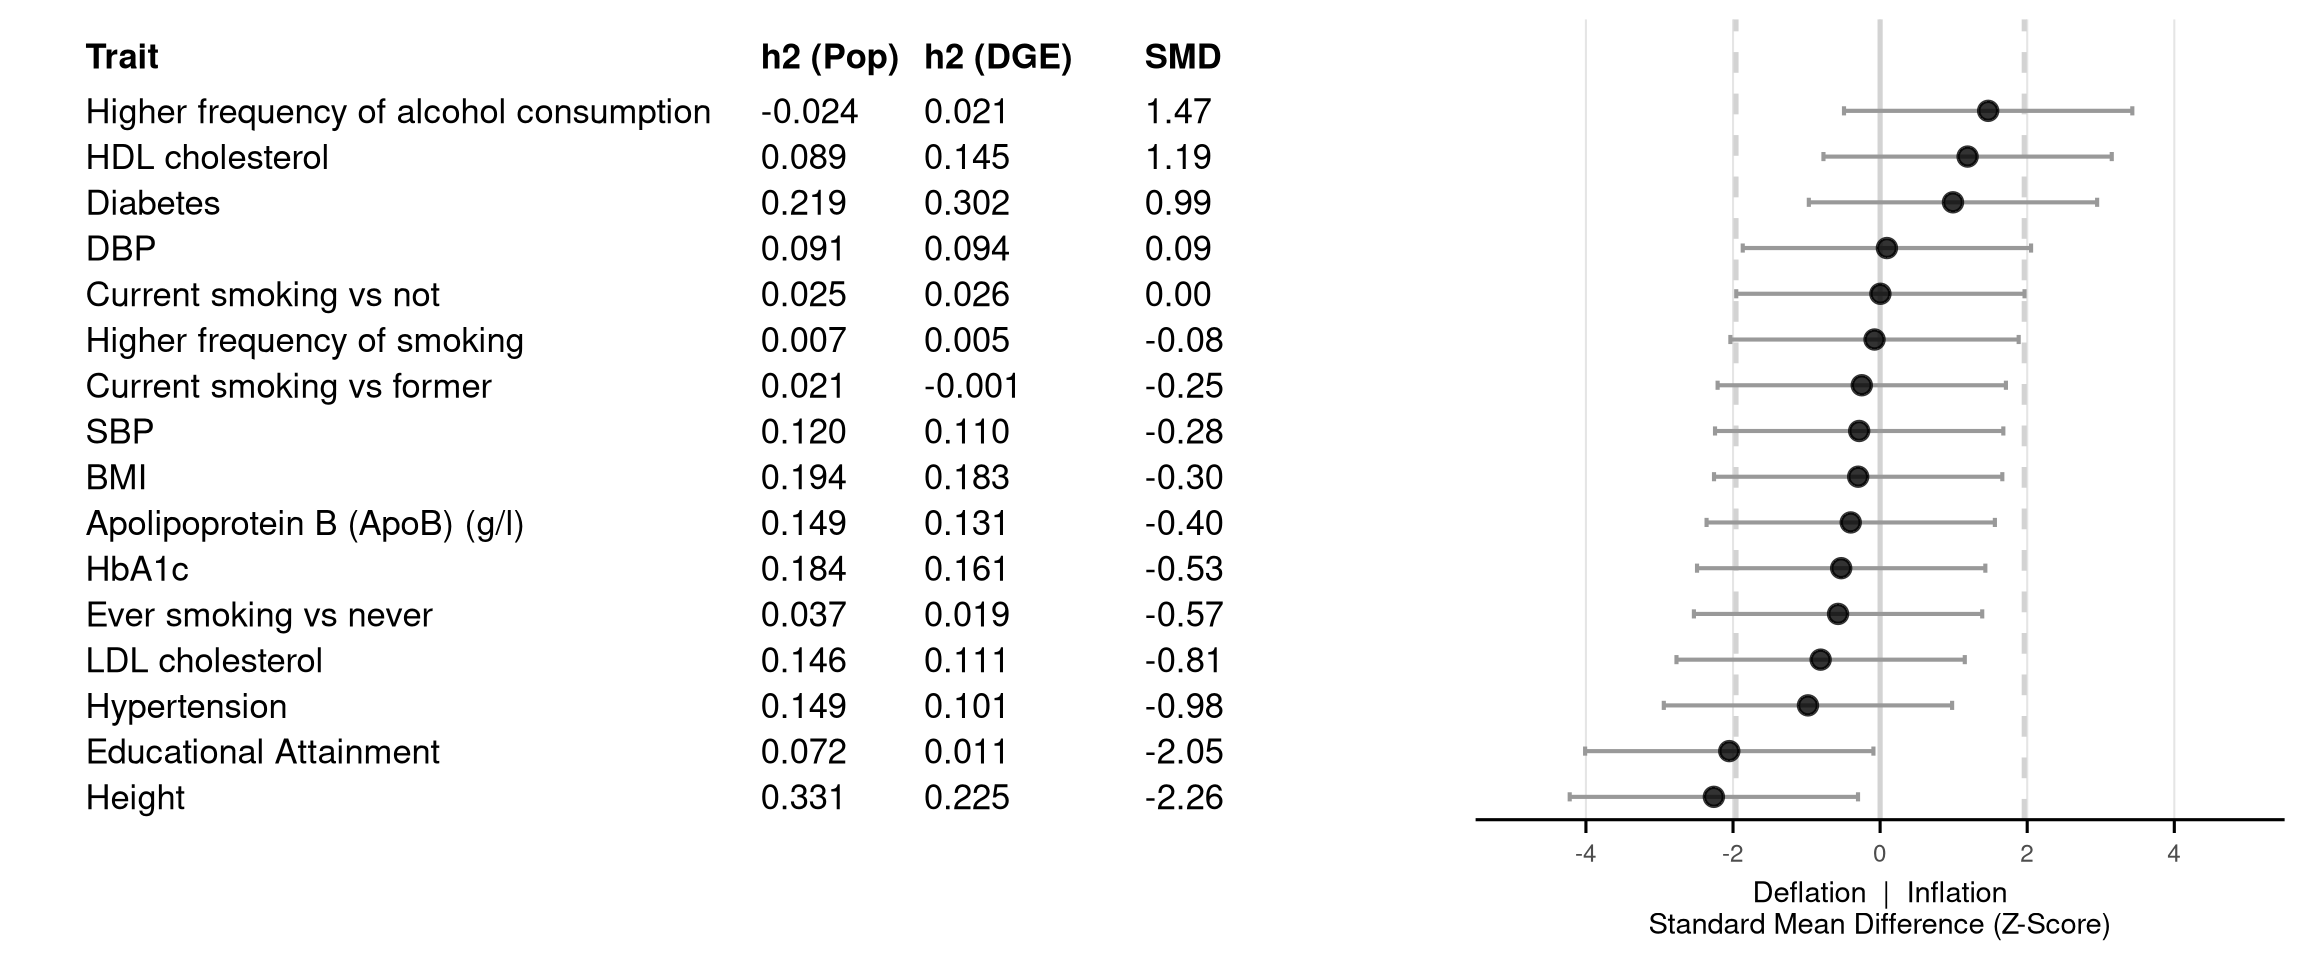
\includegraphics[width=0.9\textwidth, height=0.75\textheight, keepaspectratio]{img/results/2027-01/heritability/heritability_comparison.smd.png}
      \caption{
        \textbf{Diferencias normalizadas entre estimaciones de heredabilidad.} Las lineas verticales en la gráfica indican CI 95\%.
      }
      \label{fig:h2-smd}
  \end{figure}
\end{frame}

\begin{frame}[b]{Las subcohortes tiene diferencias sistemáticas por sesgos de averiguación}
  \begin{figure}[htpb]
      \centering
      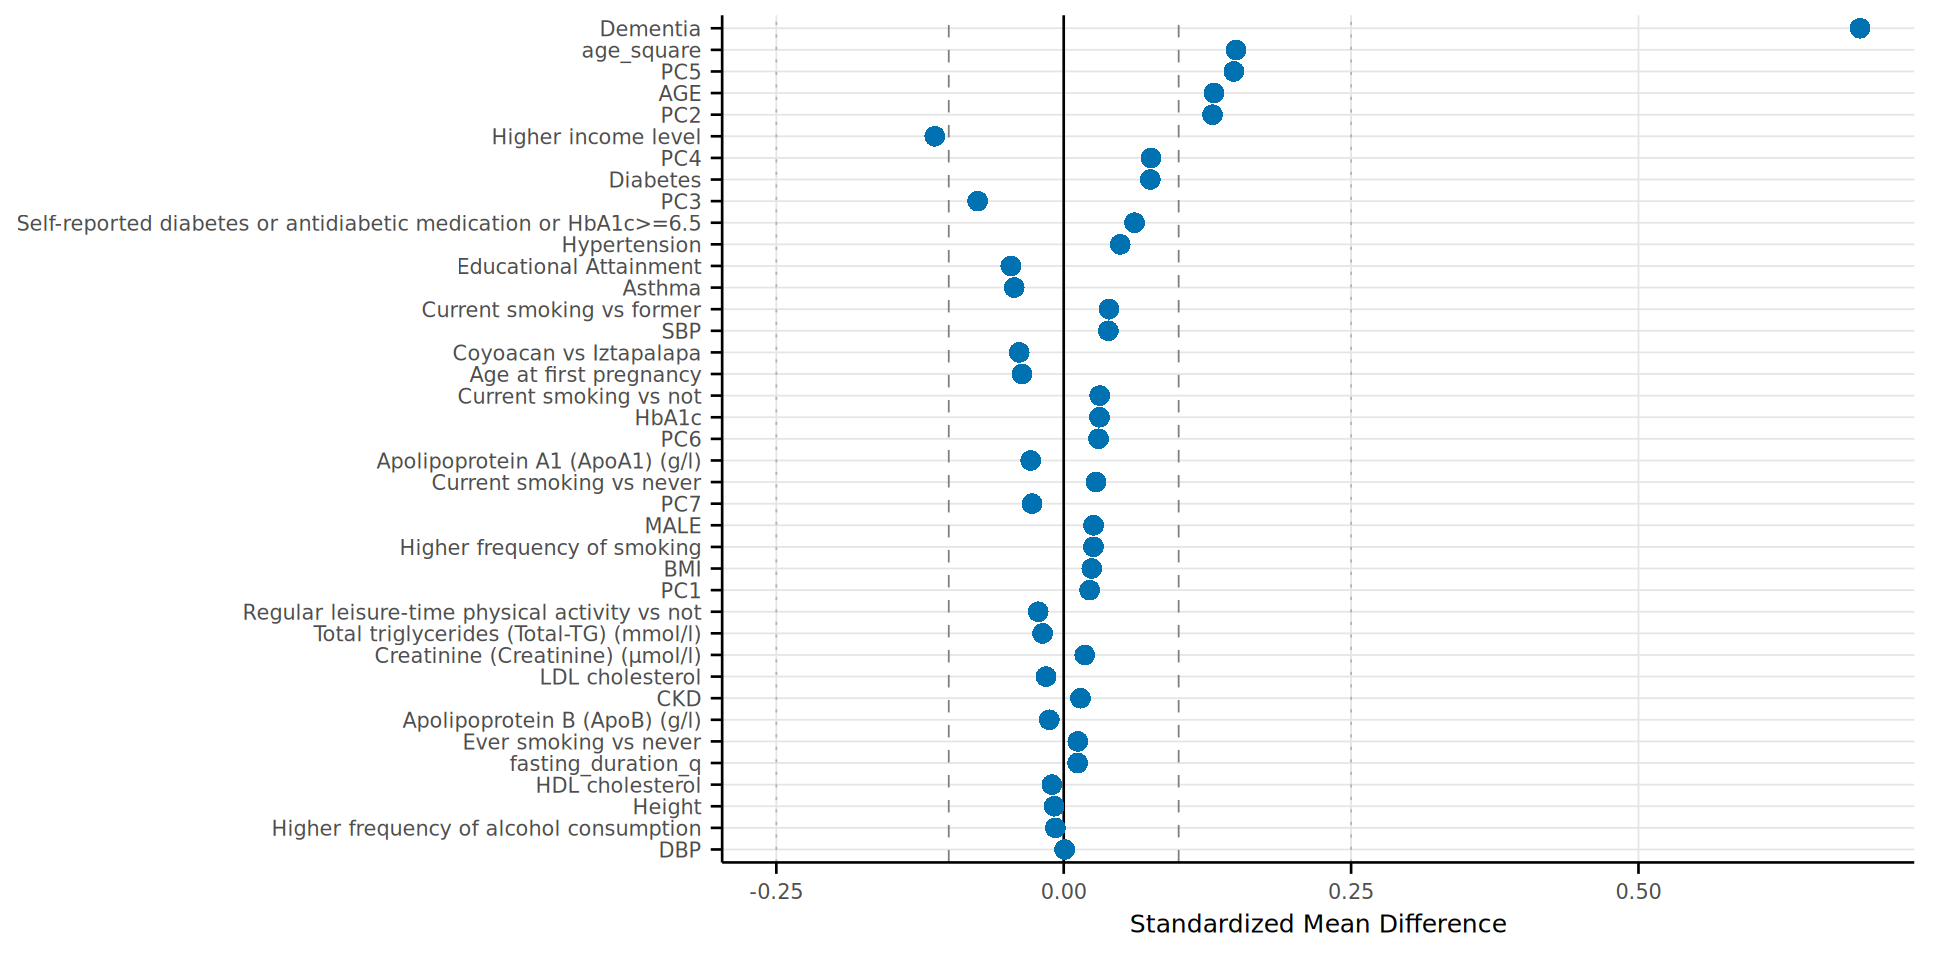
\includegraphics[width=0.9\textwidth, height=0.75\textheight, keepaspectratio]{img/results/2027-01/phenotype-smd-analyses/forest_smd_bias_assessment_cropped.png}
      \caption{
        \textbf{Diferencias por sesgos de averiguación.} Diferencias de medias estandarizadas (SMD) entre subcohortes.
      }
      \label{fig:bias_assessment}
  \end{figure}
\end{frame}

\begin{frame}[c]{Atenuación a nivel de \textit{locus} independientes (Clumping)}
  \begin{table}[htpb]
      \centering
      \resizebox{\textwidth}{!}{
      \begin{tabular}{llllrrlp{4.5cm}}
          \toprule
          \textbf{Fenotipo} & \textbf{SNP} & \textbf{Gen} & \textbf{PopGWAS} $\beta$ & \textbf{FGWAS} $\beta$ & $\Delta \beta$ & \textbf{FDR} & \textbf{Patrón de Atenuación} \\
          \midrule
          Diabetes & \texttt{chr6:20660459:G:A} & \textit{CDKAL1} & -0.178 & -0.010 & -0.168 & $1.4 \times 10^{-8}$ & \textbf{Alto:} Gran efecto poblacional; efecto directo cercano a cero. \\
          Diabetes & \texttt{chr9:22137686:T:G} & \textit{CDKN2B} & -0.163 & -0.009 & -0.154 & $5.2 \times 10^{-8}$ & \textbf{Alto:} Asociación inflada por sesgos/confusión. \\
          LDL & \texttt{chr5:156924336:T:C} & \textit{TIMD4} & -0.049 & -0.016 & -0.032 & 0.145 & \textbf{Fuerte:} Efecto directo $\sim 3\times$ menor. \\
          Estatura & \texttt{chr7:44189469:C:T} & \textit{GCK} & -0.094 & -0.077 & -0.017 & 0.899 & \textbf{Moderado:} Efecto conservado, ligera sobreestimación. \\
          HbA1c & \texttt{chr19:44908822:C:T} & \textit{APOE} & 0.498 & 0.481 & 0.017 & 0.966 & \textbf{Estable:} Efecto directo robusto, mínima confusión. \\
          \bottomrule
      \end{tabular}
      }
      \caption{
        \textbf{Resumen de atenuación en \textit{loci} representativos (PopGWAS vs FGWAS).}
      }
      \label{tab:clumping_attenuation}
  \end{table}
\end{frame}

\begin{frame}[c]{Frecuencias alélicas por ancestría continental (MCPS)}
  \begin{table}[htpb]
      \centering
      \begin{tabular}{llrrr}
          \toprule
          \textbf{Gen} & \textbf{\textit{locus}} & \textbf{Freq. IMX} & \textbf{Freq. EUR} & \textbf{$\Delta$ (IMX - EUR)} \\
          \midrule
          \textit{CDKAL1} & \texttt{chr6:20660459:G:A} & 25.6\% & 34.2\% & $-8.6\%$ \\
          \textit{CDKN2B} & \texttt{chr9:22137686:T:G} & 34.1\% & 29.8\% & $+4.3\%$ \\
          \textit{GCK} & \texttt{chr7:44189469:C:T} & 19.3\% & 20.5\% & $-1.2\%$ \\
          \textit{TIMD4} & \texttt{chr5:156924336:T:C} & 53.0\% & 30.0\% & $+23.0\%$ \\
          \bottomrule
      \end{tabular}
      \caption{
        \textbf{Frecuencias alélicas en subpoblaciones de MCPS.} IMX = Indígena Americano, EUR = Europeo. Datos extraídos del MCPS Allele Frequency Browser (\url{https://rgc-mcps.regeneron.com/home}).
      }
  \end{table}
\end{frame}

\begin{frame}[t]{Conclusiones: Relevancia de los Modelos Familiares}
  \begin{columns}[T]
      \begin{column}{0.31\textwidth}
          \begin{block}{1. Diagnóstico de Sesgos}
              Los GWAS familiares operan como herramientas diagnósticas que permiten determinar la dirección y magnitud de sesgos en diseños de descubrimiento (PopGWAS), más que como estrategias primarias para identificación de \textit{loci}.
          \end{block}
      \end{column}
      \begin{column}{0.31\textwidth}
          \begin{block}{2. Poder Estadístico en MCPS}
              La implementación del estimador robusto incrementa eficientemente el tamaño de muestra efectivo frente a alternativas intra-familiares, permitiendo documentar rigurosamente efectos de composición ambiental en la cohorte.
          \end{block}
      \end{column}
      \begin{column}{0.33\textwidth}
          \begin{block}{3. Predicción de Riesgo (PRS)}
              Históricamente, construir puntajes poligénicos con estimaciones de FGWAS no ha mejorado la precisión predictiva. Sin embargo, evaluar empíricamente esta aproximación en población mexicana es un paso necesario para consolidar la evidencia.
          \end{block}
      \end{column}
  \end{columns}
\end{frame}

\begin{frame}[c]{Ancestría y Confusión Ambiental en Diabetes}
  \begin{itemize}
      \item<1-> Diabetes mellitus: fenotipo crítico con los mayores niveles de sesgo poblacional empírico.
      \item<2-> \textcite{torres2026-diabetes, wang2025-mcps}: La ancestría mexicana explica la alta prevalencia de la enfermedad.
      \item<3-> Estimadores intrafamiliares identifican \textbf{falsos positivos} en \textit{loci} canónicos de diabetes por confusión ambiental. % ponytail: directo al grano
      \item<4-> Urge el desarrollo de herramientas genómicas de mayor precisión para México.
  \end{itemize}
\end{frame}

% % \section{Background}
\section{Antecedentes}

% =====================================
% RESULTADOS DEL SEMESTRE ANTERIOR
%   - Usamos el método de Imputación Mendeliana para 17 rasgos complejos.
%   - Nos dimos cuenta que, si bien el workflow de snipar funciona, la imputación mendeliana
%   no es adecuada para poblaciones mestizas como México.
% =====================================

% \begin{frame}[c]{Incrementar Tamaño de Muestra: Imputación Mendeliana}
%     \begin{columns}
%         % --- Mendelian Imputation ---
%         \begin{column}{0.65\textwidth}
%             \begin{figure}
%                 \centering
%                 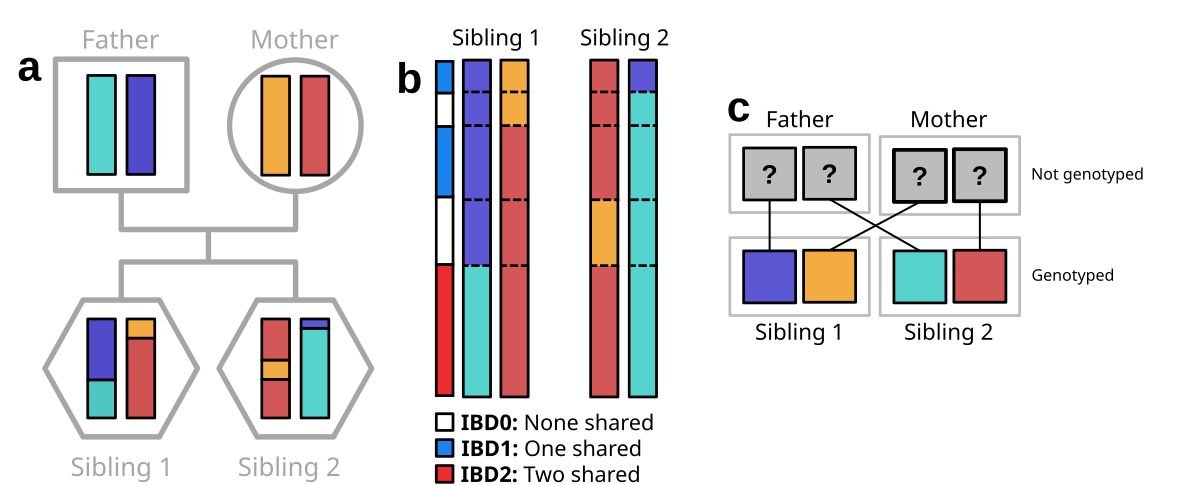
\includegraphics[width=0.9\textwidth]{img/diagrams/mendelian-imputation.png} 
%                 \caption{
%                     \textbf{El proceso de meisosis segrega aleatoriamente los alelos parentales.}
%                     (A)
%                     (B)
%                 }
%             \end{figure}
%         \end{column}
% 
%         % --- Manhattan Plot of previous results ---
%         \begin{column}{0.35\textwidth}
%             \sffamily\centering
%             \only<2->{
%                 {\small
%                     La \enquote{Imputación mendeliana} \parencite{young2022-fgwas} \textbf{introduce sesgos} en poblaciones con \textbf{mestizaje reciente}.\\[2.5pt]
%                 }
%                 {\scriptsize
%                     \textcolor{gray}{Depende de \textit{frecuencias alélicas} para algunos casos de IBD.}\\[2em]
%                 }
%             }
%             \only<3->{\small
%                 \alert{No podemos confiar} en asociaciones que usen \enquote{Imputación mendeliana} en el MCPS.\\[1em]
%             }
%             \only<4->{\small
%                 ¿Cómo incrementamos el tamaño de muestra de forma \textbf{robusta} al mestizaje reciente?
%             }
%         \end{column}
%     \end{columns}
% \end{frame}

% ============================================================
% Robust estimator
% ============================================================
% \begin{frame}[c]{Incrementar Tamaño de Muestra: Estimador robusto}
%   \begin{columns}[b]
%     % --- LEFT COLUMN: Traditional methods ---
%     \begin{column}{0.45\textwidth}
%       \centering
%       {\footnotesize
%         % Traditional methods like \textcite{benyamin2009-fgwas,howe2022-sibdiff,young2022-fgwas}.
%         Métodos de FGWAS convencionales \parencite{benyamin2009-fgwas,howe2022-sibdiff,young2022-fgwas}.
%       }\\[1.5em]
%       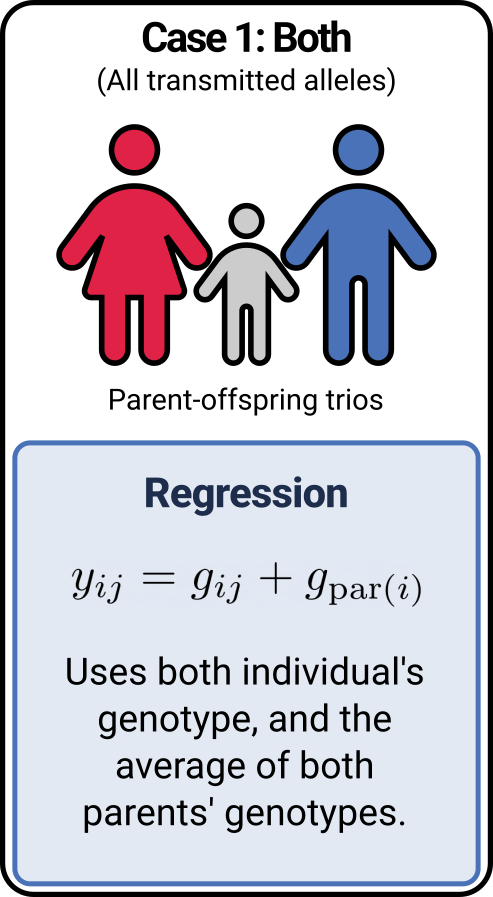
\includegraphics[height=4cm]{img/diagrams/robust-estimator/case-01.png}
%       
%       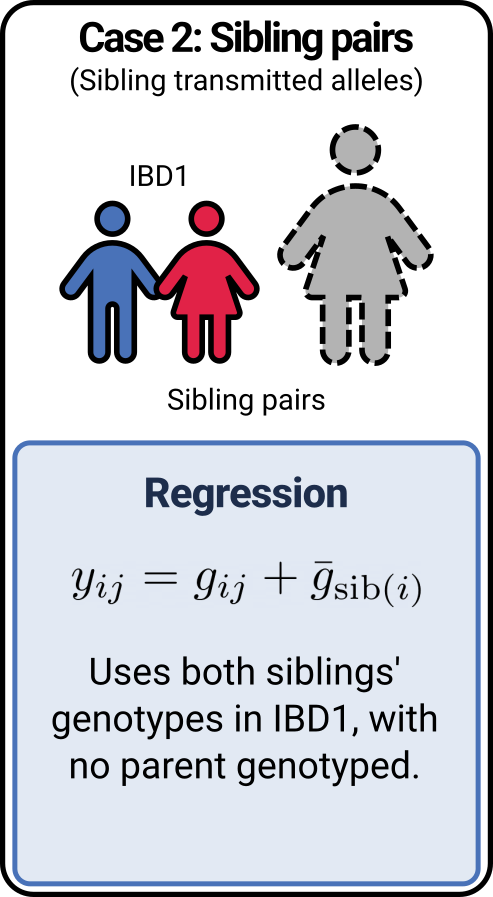
\includegraphics[height=4cm]{img/diagrams/robust-estimator/case-02.png}
%     \end{column}
% 
%     \pause
% 
%     % --- RIGHT COLUMN: Robust estimator ---
%     \begin{column}{0.45\textwidth}
%       \centering
%       %
%       {\footnotesize
%         % The \textit{robust estimator} by \textcite{guan2025-fgwas} \textbf{increases} effective sample size ($N_{\mathrm{eff}}$) and it is robust to \textbf{recent admixture}.
%         El \enquote{estimador robusto} \parencite{guan2025-fgwas} \textbf{incrementa} el tamaño efectivo de muestra, siendo robusto a \textit{mestizaje reciente}.
%       }\\[1.5em]
%       %
%       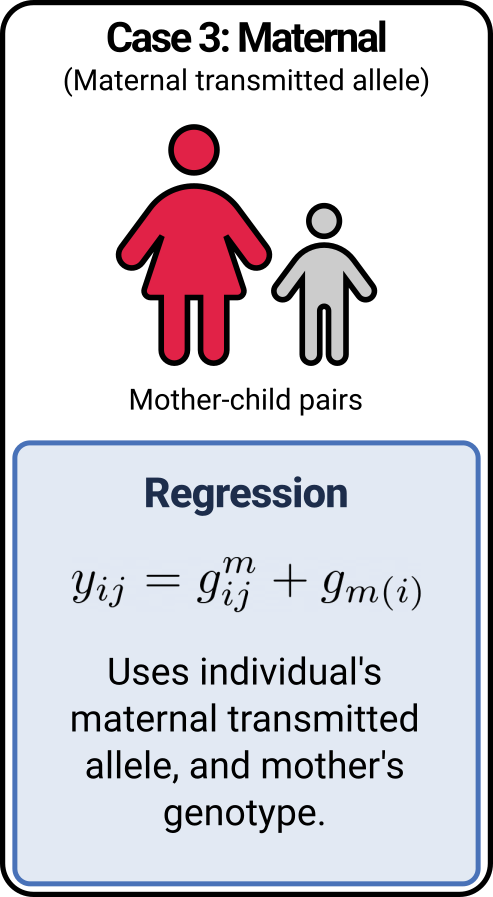
\includegraphics[height=4cm]{img/diagrams/robust-estimator/case-03.png}
%       \hspace{1em}
%       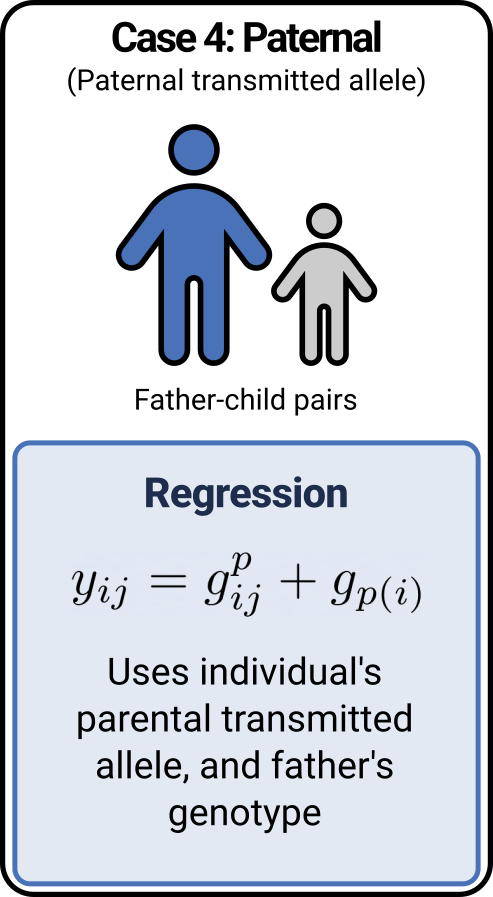
\includegraphics[height=4cm]{img/diagrams/robust-estimator/case-04.png}
%     \end{column}
%   \end{columns}
% \end{frame}

\begin{frame}[c]{Incrementando poder estadístico: Estimador robusto}
    \vspace{1em}
    \begin{columns}[c]
        % --- Column A ----
        \begin{column}{0.35\textwidth}
            \textbf{Cambio de estrategia...}\\[1em]
            \footnotesize
            \begin{itemize}
                \item<1-> La \textit{Imputación Mendeliana} \parencite{young2022-fgwas} es sensible a \textbf{frecuencias alélicas}.
                \item<2-> En cohortes con mestizaje reciente ---como el MCPS--- la \textit{Imputación Mendeliana} puede introducir sesgos.
                \item<3-> El \textit{Estimador Robusto} de \textcite{guan2025-fgwas} expande el tamaño de muestra para FGWAS, siendo robusto a mestizaje reciente.
            \end{itemize}
        \end{column}

        % --- Column B ----
        \begin{column}{0.70\textwidth}<4->
            \centering
            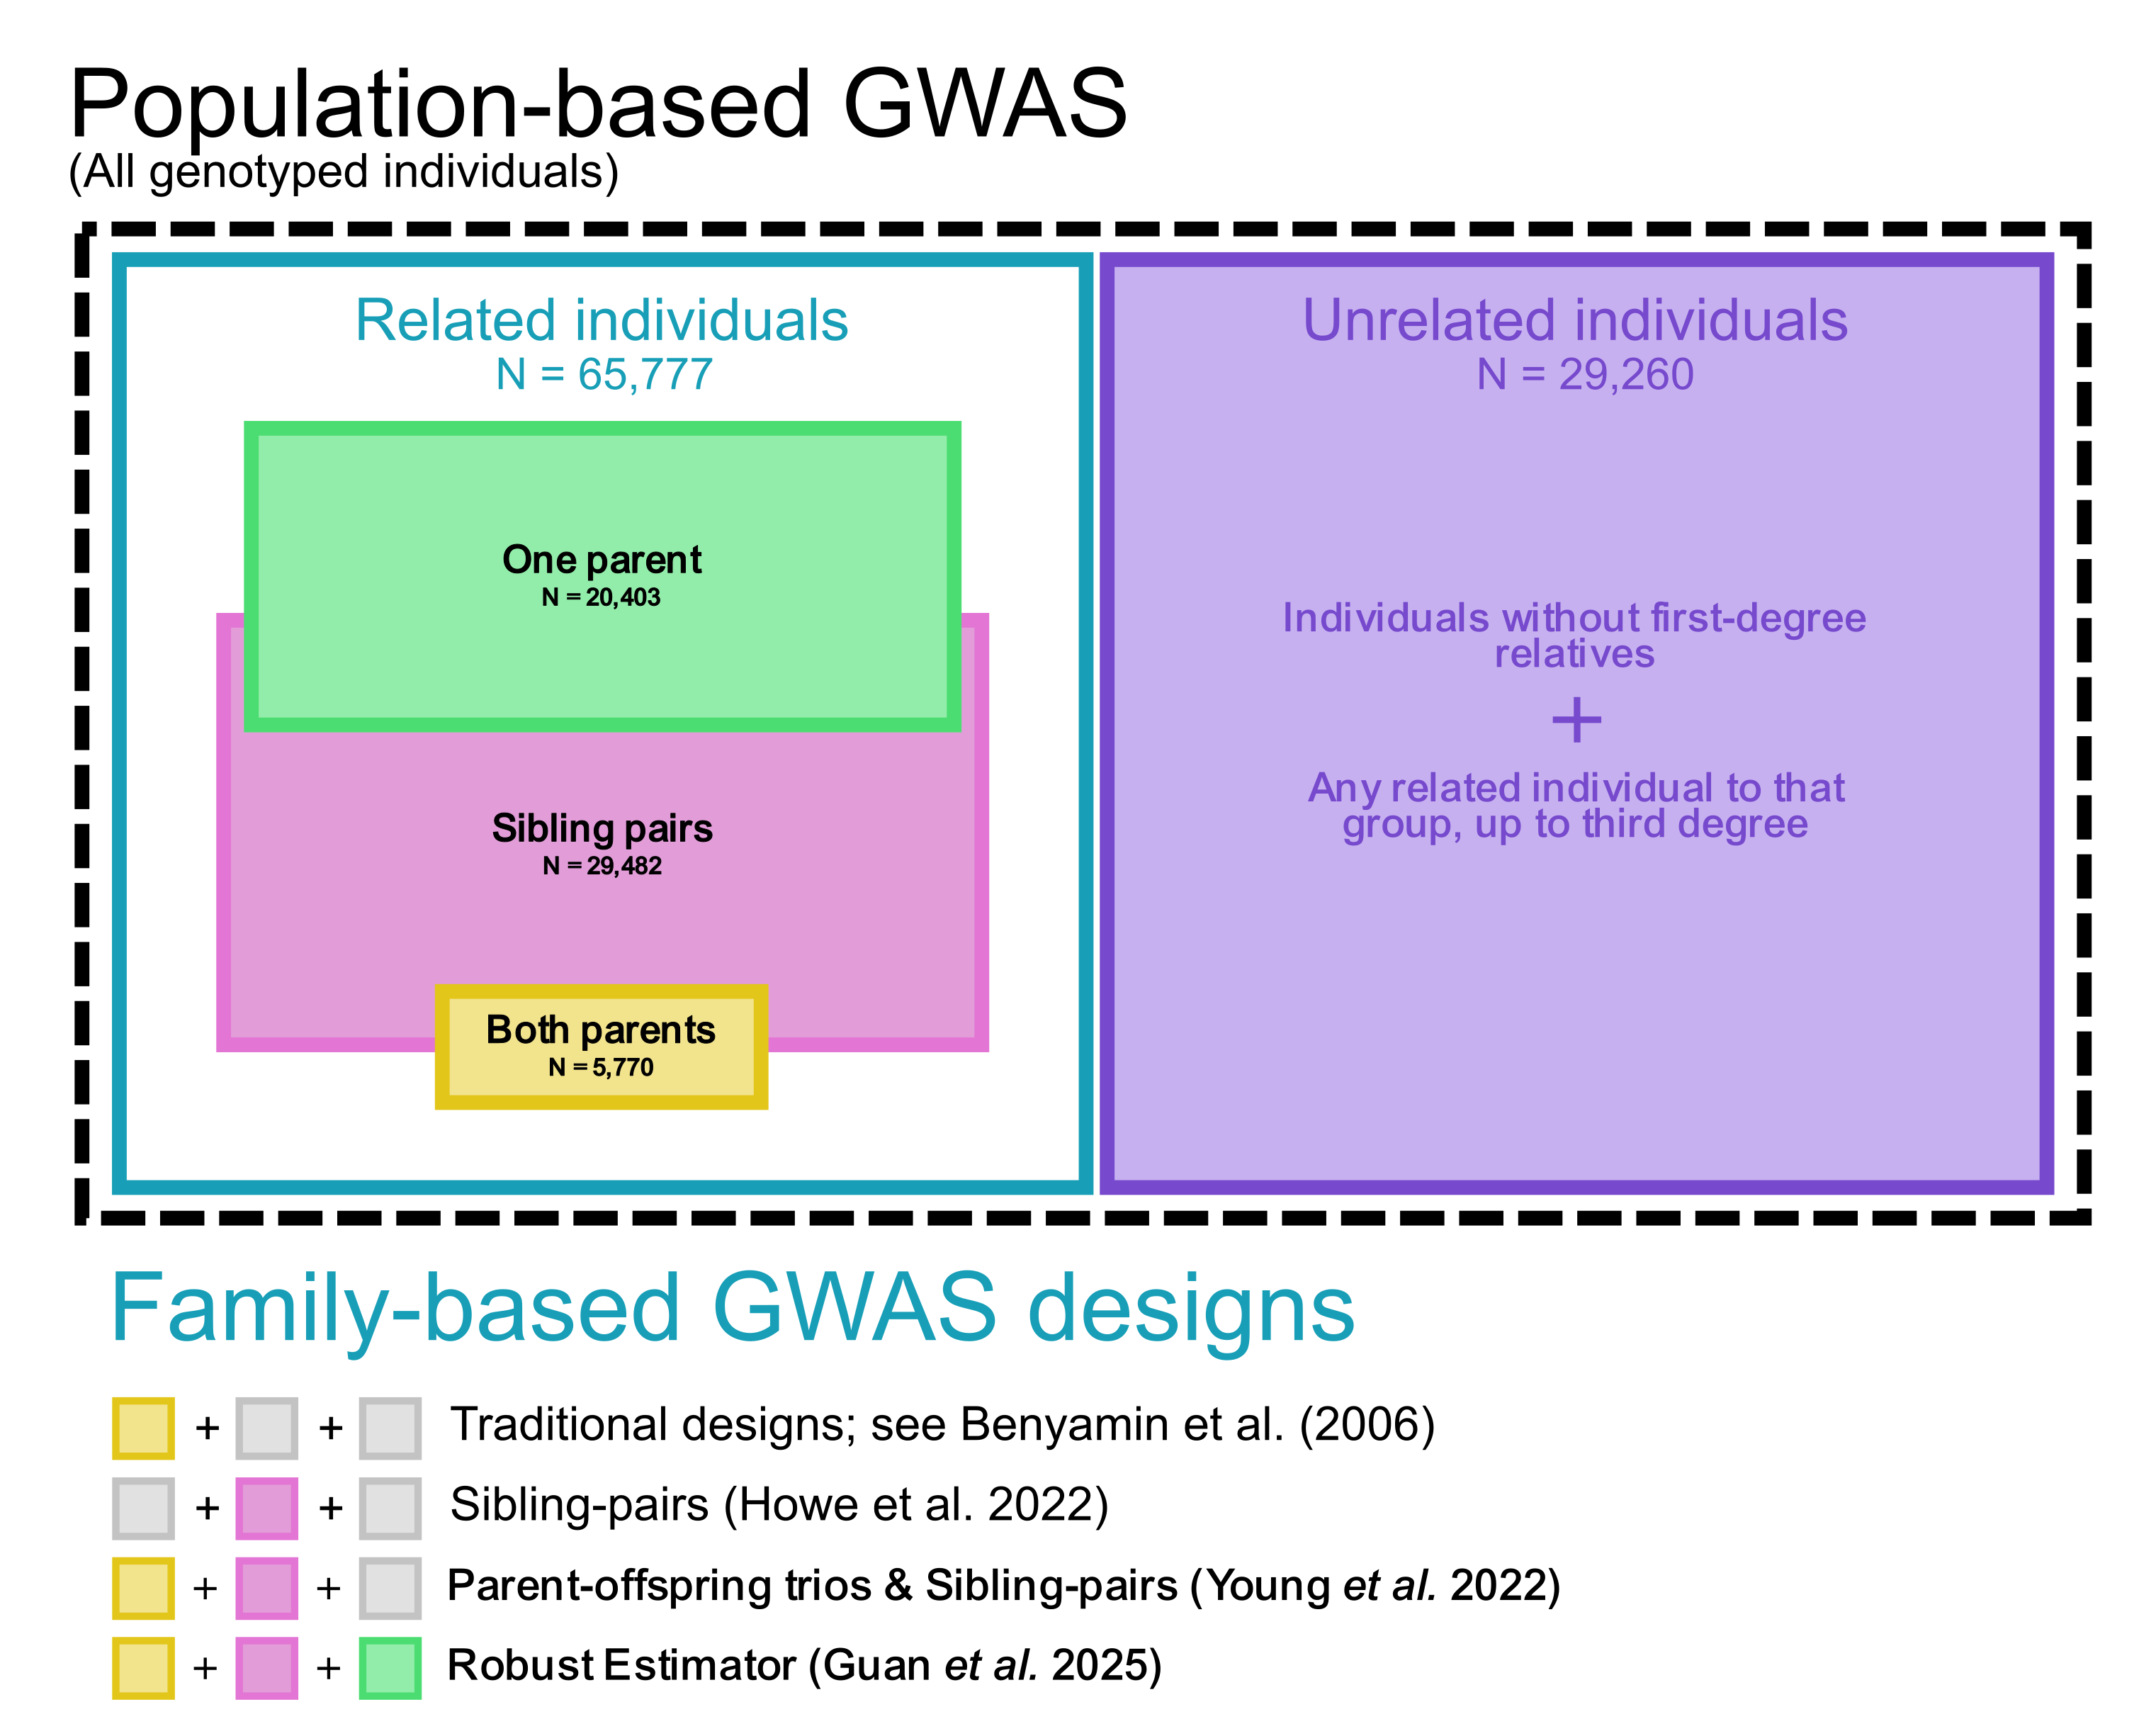
\includegraphics[width=0.80\textwidth]{img/diagrams/robust-estimator_neff.png}
        \end{column}
    \end{columns}
\end{frame}
% % \section{Objectives}
\section{Objetivos}

% --- OBJETIVO PRINCIPAL ---
\begin{frame}[c]{Objectivos de investigación (Doctorado)}
  \begin{center}
    % --- Objectivo principal del doctorado ---
    {\sffamily\bfseries\Large\color{ccgblue}
      Objetivo principal
    }\\[0.25cm]
    {\sffamily\large
      Estimar \textbf{efectos genéticos directos (DGEs)} para una amplia gama de rasgos complejos
      y enfermedades en una cohorte \textit{mexicana}, utilizando el MCPS y nuevos estimadores
      FGWAS para aumentar drásticamente el poder estadístico típicamente limitada
      en diseños familiares.
    }
    \vfill
    % --- Hipótesis principal ---
    \uncover<2->{
      {\sffamily\bfseries\Large\color{ccgblue}
        Hipótesis principal
      }\\[0.25cm]
      {\sffamily\large

        % --- Resumen para presentacion ---
        Para la población mestiza del MCPS, un FGWAS con estimador robusto 
        a mestizaje reciente cuantificará DGEs en múltiples
        rasgos complejos, superando otros diseños para identificar
        falsos-positivos de PopGWAS y revelar nuevos \textit{loci} ocultos.

        % % --- Traduccion directa ----
        % Para la población con mestizaje reciente del
        % Estudio Prospectivo de la Ciudad de México (MCPS, por sus siglas en inglés),
        % el FGWAS de estimador robusto proveerá estimaciones
        % de efectos genéticos directos (DGEs) en para una selección
        % comprensiva de rasgos complejos y enfermedades,
        % dando un incremento substancial comparado a otros diseños de FGWAS
        % lo que nos ayudará a identificar falsos-positivos en PopGWAS
        % y potencialmente nuevos \textit{loci} ocultos.

        % % --- Original ---
        % For the recently admixed genomes of the Mexico City Prospective Study (MCPS), the FGWAS robust estimator will
        % provide unbiased estimates of direct genetic effects (DGEs) across a comprehensive set of complex traits and diseases,
        % yielding a substantial gain in effective sample size and statistical power relative to other FGWAS frameworks, identify
        % false-positive effect sizes in PopGWAS, and identify novel loci hidden to PopGWAS.
      }
    }

  \end{center}
\end{frame}

% --- OBJETIVOS ESPECÍFICOS DE INVESTIGACIÓN ---
\begin{frame}[c]{Objetivos específicos}
  
  % 1. Obtener asociaciones genéticas libres de sesgos para 200 rasgos complejos. Y ampliar su poder estadístico con el 'estimador robusto'
  % 2. Cuantificar cuáles son los más suceptibles a efectos de confusión.
  % 3. Realizar comparaciones con otras cohortes mexicanas y globales.
  % 4. Realizar análisis posteriores priorizando genes candidatos, predecir riesgo poligénico (PGS) e inferir causalidad (randomización mendeliana).
  % 5. Desarrollar una plataforma en línea de libre acceso para garantizar la utilidad e interpretabilidad de los resultados.

  \begin{center}
      \resizebox{\textwidth}{!}{%
      \begin{tikzpicture}[
          % 1. Configuración de la caja base
          box/.style={
              rectangle,
              rounded corners=4mm,
              very thick,
              align=center,
              font=\sffamily\bfseries\large,
              minimum width=5.2cm,
              minimum height=2cm,
              inner sep=8pt
          },
          % 2. Configuración de estilos activos con las nuevas variables
          active1/.style={fill=bluefill, draw=bluestroke, text=bluestroke!50!black},
          active2/.style={fill=grayfill, draw=graystroke, text=graystroke!50!black},
          active3/.style={fill=greenfill, draw=greenstroke, text=greenstroke!50!black},
          active4/.style={fill=yellowfill, draw=yellowstroke, text=yellowstroke!50!black},
          active5/.style={fill=purplefill, draw=purplestroke, text=purplestroke!50!black},
          % 3. AMBIENTE PERSONALIZADO: Estilo inactivo usando variables aqua
          inactive/.style={fill=aquafill, draw=aquastroke, text=aquastroke},
          % 4. Configuración de flechas como figuras
          arrow_base/.style={single arrow, fill=aquastroke!30, minimum height=0.8cm, single arrow head extend=2.5mm},
          arrow_right/.style={arrow_base, shape border rotate=0},
          arrow_down/.style={arrow_base, shape border rotate=270},
          arrow_left/.style={arrow_base, shape border rotate=180}
      ]

      % === FILA SUPERIOR (Izquierda a Derecha) ===
      
      % Objetivo 1
      \node[box, active1] (o1) {1. Asociaciones Genéticas\\[2mm] \small\normalfont (Estimador robusto)};
      
      % Flecha 1
      \node[arrow_right, right=0.3cm of o1] (a1) {};
      
      % Objetivo 2
      \node[box, active2, right=0.3cm of a1] (o2) {2. Comparación de efectos\\[2mm] \small\normalfont (Cuantificación de sesgos)};
      
      % Flecha 2
      \node[arrow_right, right=0.3cm of o2] (a2) {};
      
      % Objetivo 3
      \node[box, inactive, right=0.3cm of a2] (o3) {3. Meta-análisis con cohortes\\[2mm] \small\normalfont (Mexicanas y globales)};

      % === CONEXIÓN HACIA ABAJO ===
      
      % Flecha 3 (Apunta hacia abajo desde el Objetivo 3)
      \node[arrow_down, below=0.3cm of o3] (a3) {};

      % === FILA INFERIOR (Derecha a Izquierda) ===
      
      % Objetivo 4 (Estilo inactivo)
        \node[box, inactive, below=0.3cm of a3] (o4) {4. Análisis posteriores\\[2mm] \small\normalfont (PGS y MR)};
      
      % Flecha 4 (Apunta hacia la izquierda)
      \node[arrow_left, left=0.3cm of o4] (a4) {};
      
      % Objetivo 5 (Estilo inactivo)
      \node[box, inactive, left=0.3cm of a4] (o5) {5. Plataforma Interactiva\\[2mm] \small\normalfont (Libre acceso)};

      \end{tikzpicture}%
      }
  \end{center}
\end{frame}

% --- OBJETIVOS DEL SEMESTRE ---
\begin{frame}[c]{Objetivos de investigación (Semestre 2026-02)}
  \sffamily\small
  \renewcommand{\arraystretch}{2.0}   % instead of 0.9
  \begin{tabular}{p{0.45\textwidth} p{0.45\textwidth}}
    \multicolumn{1}{c}{\cellcolor{ccgblue}{\textcolor{white}{\large\bfseries Objetivos}}} & 
    \multicolumn{1}{c}{\cellcolor{ccgblue}{\textcolor{white}{\large\bfseries Resultados esperados}}} \\

    1. Obtener DGEs para 17 rasgos complejos del MCPS, usando el \textit{estimador robusto} \parencite{guan2025-fgwas}. &
    El \textit{estimador robusto} \parencite{guan2025-fgwas} produce DGEs con tamaños de muestra efectiva \textbf{más grandes} que otros métodos de FGWAS, y más que en el UKB. \\

    2. Comparar heredabilidad de DGEs y efectos poblacionales en cada rasgo para determinar la \textbf{dirección de atenuación} de los efectos de confusión. &
    Heredabilidad inferida con DGEs será \textbf{más pequeña} que la de efectos poblacionales de la misma cohorte. \\

    3. Cuantificar la magnitud de sesgos mediante correlaciones entre DGEs y efectos poblacionales. &
    Las correlaciones serán \textbf{substancialmente más pequeños} en rasgos complejos con un alto nivel de confusión/sesgo.
  \end{tabular}
\end{frame}
% % \section{Methodology}
\section{Metodología}

% Define custom colors for the workflow diagram
\definecolor{datafill}{HTML}{E3F2FD}
\definecolor{datastroke}{HTML}{2196F3}
\definecolor{subsetfill}{HTML}{E0F2F1}
\definecolor{subsetstroke}{HTML}{009688}
\definecolor{processfill}{HTML}{F5F5F5}
\definecolor{processstroke}{HTML}{9E9E9E}
\definecolor{gwasfill}{HTML}{E8F5E9}
\definecolor{gwasstroke}{HTML}{4CAF50}
\definecolor{postfill}{HTML}{FFF3E0}
\definecolor{poststroke}{HTML}{FF9800}
\definecolor{vizfill}{HTML}{F3E5F5}
\definecolor{vizstroke}{HTML}{9C27B0}

% =============================
% FLUJO DE TRABAJO COMPLETO
% =============================
\begin{frame}{Flujo de trabajo completo}
  \begin{columns}[c]
    % --- WORKFLOW DETAILS ---
    \begin{column}{0.45\textwidth}
      % --- Text --- 
      {\footnotesize\sffamily
        \begin{itemize}
          \item<2-> \textcolor{datastroke}{\textbf{Datos de entrada:}} Mismos fenotipos y genotipos (imputados y arreglos chip) que el semestre pasado.
          \item<3-> \textcolor{subsetstroke}{\textbf{Diseño experimental para comparaciones:}} Asegurar \textit{independencia} estadística entre $\hat{\delta}$ y $\hat{\beta}$ usando \textbf{individuos no emparentados} (unrelated).
          \item<4-> \textcolor{gwasstroke}{\textbf{GWAS:}} FGWAS ($\hat{\delta}$) con \textit{snipar} \parencite{young2022-fgwas,guan2025-fgwas} y GWAS ($\hat{\beta}$) con REGENIE \parencite{mbatchou2021-regenie}.
          \item<5-> \textcolor{poststroke}{\textbf{Análisis posteriores:}} Correlación entre estimadores con \textit{snipar} \parencite{young2022-fgwas} y heredabilidad/correlaciones genéticas con LDSC \parencite{bulik-sullivan2015-ldsc}.
        \end{itemize}
      }
    \end{column}

    % --- COMPLETE WORKFLOW DIAGRAM ---
    \begin{column}{0.55\textwidth}
      \centering
      \resizebox{!}{5.5cm}{
        \begin{tikzpicture}[
            box/.style={rectangle, thick, rounded corners, align=center, minimum height=0.8cm, inner sep=0.2cm},
            data/.style={box, fill=datafill, draw=datastroke},
            subset/.style={box, fill=grayfill, draw=graystroke},
            process/.style={box, fill=aquafill, draw=aquastroke},
            gwas/.style={box, fill=greenfill, draw=greenstroke},
            post/.style={box, fill=yellowfill, draw=yellowstroke},
            viz/.style={box, fill=purplefill, draw=purplestroke},
            arrow/.style={->, thick, >=stealth, draw=gray!80!black}
          ]
          
          % Nodes
          \node[data] (Raw) at (0,0) {Raw Data\\(Phenotypes \& Genotypes)};
          \node[process] (Prep) at (0,-1.5) {00: Input Processing\\(QC \& Subsetting)};
          
          \node[subset] (Fams) at (-3.5,-3.0) {All Individuals};
          \node[subset] (Unrel) at (3.5,-3.0) {Unrelated Individuals};
          
          \node[gwas] (Snipar) at (-3.5,-4.5) {01: SNIPAR\\(Robust Estimator)};
          \node[gwas] (Regenie) at (3.5,-4.5) {01: REGENIE\\(Two-step GWAS)};
          
          \node[post] (Jack) at (-3.5,-6.0) {02: SNIPAR\\(Jackknife Correlation)};
          \node[post] (LDSC) at (3.5,-6.0) {02: LDSC\\(Heritability \&\\Genetic Correlation)};
          
          \node[viz] (Viz) at (0,-7.5) {03: Visualization\\(Manhattan, QQ, \& Effect Size Plots)};
          
          % Edges
          \draw[arrow] (Raw) -- (Prep);
          \draw[arrow] (Prep) -- (Unrel);
          \draw[arrow] (Prep) -- (Fams);
          
          \draw[arrow] (Unrel) -- (Regenie);
          \draw[arrow] (Fams) -- (Snipar);
          
          \draw[arrow] (Regenie) -- (LDSC);
          \draw[arrow] (Regenie) -- (Jack);
          \draw[arrow] (Snipar) -- (LDSC);
          \draw[arrow] (Snipar) -- (Jack);
          
          \draw[arrow] (LDSC) -- (Viz);
          \draw[arrow] (Jack) -- (Viz);
          
        \end{tikzpicture}
      }
    \end{column}
  \end{columns}
\end{frame}

% ============================================================
% Phenotype and Genotype data
% ============================================================
\begin{frame}[fragile]{Datos de entrada: Fenotipos} % <-- 1. Added [fragile]
  \sffamily
  \begin{columns}[c]
    % --- Text ---
    \begin{column}{0.55\textwidth}

        {\small
        Estandarización de \textbf{fenotipos} y \textbf{covariantes} (age, age2, sex, PC1-7) respecto al \textit{GWAS Atlas} de MCPS para mejor comparabilidad\\[2pt]
        }

        \begin{columns}[T]
            % --- Beheavioural traits ----
            \begin{column}{0.45\textwidth}
              \begin{exampleblock}{Behavioural}
              \scriptsize
              \begin{enumerate}
                \item Educational attainment
                \item Age of first pregnancy
                \item Income level
                \item Smoking vs. never
                \item Current smoking vs. not
                \item Current smoking vs. former
                \item Frequency of smoking
                \item Frequency of alcohol
              \end{enumerate}
              \end{exampleblock}
            \end{column}
            % --- Clinical traits ----
            \begin{column}{0.45\textwidth}
              \begin{block}{Biomedical}
              \scriptsize
              \begin{enumerate}
                \item Asthma
                \item Systolic Blood Pressure (SBP)
                \item Diastolic Blood Pressure (SBP)
                \item Height
                \item Body-Mass Index (BMI)
                \item \textit{Clinical} LDL Cholesterol (LDL)
                \item HDL Cholesterol (HDL)
                \item Self-reported hypertension
                \item Self-reported diabetes
              \end{enumerate}
              \end{block}
            \end{column}
        \end{columns}
    \end{column}

    % --- Flow Chart and Photos ---
    \begin{column}{0.35\textwidth}
      \centering % <-- 2. Moved \centering outside to center the whole column contents
      \resizebox{!}{3cm}{
        \begin{tikzpicture}[
          % Base node styles
          box/.style={rectangle, thick, rounded corners, align=center, minimum height=0.8cm, inner sep=0.2cm},
          % Specific styles based on the image's color scheme
          db/.style={box, fill=green!10, draw=green!60!black, text width=2.8cm}, % Database representation
          process/.style={box, fill=white, draw=gray!80, text width=3cm},
          greendoc/.style={box, fill=green!10, draw=green!50, text width=2.4cm},
          purpledoc/.style={box, fill=purple!10, draw=purple!50, text width=2.4cm},
          % Grouping styles
          groupbox/.style={rectangle, draw=black, thick, inner sep=0.4cm, rounded corners},
          grouplabel/.style={fill=black, text=white, font=\sffamily\bfseries\scriptsize, rounded corners=2pt, inner sep=3pt},
          % Arrow styles
          greendotted/.style={->, ultra thick, dotted, draw=green!50, >=stealth},
          greenarrow/.style={->, ultra thick, draw=green!50, >=stealth},
          purplearrow/.style={->, ultra thick, draw=purple!50, >=stealth}
        ]
          % ==========================================
          % 1. Top Section: Data Source
          % ==========================================
          \node[db] (std_pheno) at (0,0) {Standardized\\phenotypes};
              
          % Background grouping box for Data Source
          \begin{scope}[on background layer]
            \node[groupbox, fit=(std_pheno), minimum width=6cm] (top_box) {};
          \end{scope}
        
          % ==========================================
          % 2. Middle Section: Scripts / Processing
          % ==========================================
          \node[process] (create_files) at (0,-2.5) {Create\\individual files};
        
          % ==========================================
          % 3. Bottom Section: Outputs
          % ==========================================
          \node[greendoc] (pheno) at (-1.8,-5) {Phenotypes};
          \node[purpledoc] (covar) at (1.8,-5) {Covariates};
        
          % Background grouping box for Scripts
          \begin{scope}[on background layer]
            \node[groupbox, fit=(create_files) (pheno) (covar), minimum width=6cm] (scripts_box) {};
            \node[grouplabel, anchor=south west] at ([xshift=0.3cm, yshift=-0.15cm]scripts_box.north west) {Scripts};
          \end{scope}
        
          % ==========================================
          % 4. Edges & Flow Routing
          % ==========================================
          % Dotted input from standardized phenotypes
          \draw[greendotted] (std_pheno) -- (create_files);
        
          % Branching solid outputs to Phenotypes and Covariates
          \draw[greenarrow] (create_files.south) -- ++(0,-0.6) -| (pheno.north);
          \draw[purplearrow] (create_files.south) -- ++(0,-0.6) -| (covar.north);
        \end{tikzpicture}
      }
      
      \vspace{10pt}
      
      % ---- Collaborators -----
      \resizebox{!}{1cm}{
        \mbox{ % <-- Wrapped the cards in an \mbox to safely group them horizontally for \resizebox
          \collabcard{img/tutors/diego-ramirez.png}{0.6cm}
            {PhD. Diego Aguilar Ramírez}
            {Intermediate Research Fellow}
            {CTSU, NDPH -- University of Oxford}
          \hspace{0.5em}
          \collabcard{img/tutors/erini-trichia.png}{0.6cm}
            {PhD. Erini Trichia}
            {Senior Statistical Epidemiologist}
            {CTSU, NDPH -- University of Oxford}
        }
      }
    \end{column}
  \end{columns}
\end{frame}

\begin{frame}[c, fragile]{Datos de entrada: Genotipos}
  \small\sffamily
  \begin{columns}
    % --- Column A ---
    \begin{column}{0.45\textwidth}
      \textbf{TOPMed-imputed} y \textbf{GSAv2-CHIP} faseados previamente por MCPS
      con \textit{SHAPEIT-4/5}\\[1em]
      \textcite{young2022-fgwas} recomiendan \textbf{INFO $\geq$ 0.99}\\[1em]
      \textbf{TOPMed-imputed} y \textbf{GSAv2-CHIP} convertidos a BGEN con \textit{plink2} para mejor compatibilidad\\[2pt]

      {\footnotesize\color{lightgray}
        \begin{itemize}
          \item Solo SNPs
          \item Eliminar variantes duplicadas
          \item GENO $\geq$ 5\%
          \item MAF $\geq$ 1\%
        \end{itemize}
      }

      \vspace{1em}
      {\bfseries GSAv2-CHIP} 341,441 variantes (140,829 individuos)\\
      {\bfseries TOPMed-Imputed} 1,076,402 variantes (140,829 individuos)
    \end{column}

    % --- Column B ---
    \begin{column}{0.50\textwidth}
      \centering
      % ---- Diagram -----
      \resizebox{0.95\textwidth}{!}{
        \begin{tikzpicture}[
            % Base node styles
            box/.style={rectangle, thick, rounded corners, align=center, minimum height=0.8cm, inner sep=0.2cm},
            % Specific styles for datasets based on the image
            gsadata/.style={box, fill=blue!10, draw=blue!50, text width=2.8cm},
            topmeddata/.style={box, fill=orange!10, draw=orange!50, text width=2.8cm},
            % Process and grouping styles
            process/.style={box, fill=white, draw=gray!80, text width=3.2cm},
            groupbox/.style={rectangle, draw=black, thick, inner sep=0.3cm, rounded corners},
            grouplabel/.style={fill=black, text=white, font=\sffamily\bfseries\scriptsize, rounded corners=2pt, inner sep=3pt},
            % Arrow styles
            bluearrow/.style={->, ultra thick, draw=blue!50, >=stealth},
            bluedotted/.style={->, ultra thick, dotted, draw=blue!50, >=stealth},
            orangearrow/.style={->, ultra thick, draw=orange!50, >=stealth},
            orangedotted/.style={->, ultra thick, dotted, draw=orange!50, >=stealth}
          ]
          
          % ==========================================
          % 1. Top Section: MCPS Data
          % ==========================================
          \node[gsadata] (gsa) at (0,0) {GSAv2\\(Phased)};
          \node[topmeddata] (topmed) at (5.5,0) {TOPMed\\(Phased)};
          
          % Background grouping box for MCPS Data
          \begin{scope}[on background layer]
            \node[groupbox, fit=(gsa) (topmed), minimum height=2.2cm] (mcps_box) {};
            % Labels overlapping the border
            \node[grouplabel, anchor=south west] at ([xshift=0.3cm, yshift=-0.15cm]mcps_box.north west) {MCPS Data};
          \end{scope}
        
          % ==========================================
          % 2. Middle Section: Tools & Processing
          % ==========================================
          % BCFTools node
          \node[process] (info) at (5.5,-2.5) {\textbf{INFO $\geq$ 0.99}\\ \footnotesize (Young et al.)};
          \begin{scope}[on background layer]
            \node[groupbox, fit=(info)] (bcf_box) {};
            \node[grouplabel, anchor=south west] at ([xshift=0.3cm, yshift=-0.15cm]bcf_box.north west) {BCFTools};
          \end{scope}
          
          % plink2 node and filter list
          \node[process] (vcf2bgen) at (0,-2.5) {VCF to BGEN};
          % \node[align=left, font=\footnotesize\color{gray!80!black}, anchor=north] (filters) at (0, -4.2) {
          %     \begin{tabular}{l}
          %       \textbullet~Solo SNPs \\
          %       \textbullet~Eliminar duplicadas \\
          %       \textbullet~GENO $\geq$ 5\% \\
          %       \textbullet~MAF $\geq$ 1\%
          %     \end{tabular}
          % };
          
          \begin{scope}[on background layer]
            % \node[groupbox, fit=(vcf2bgen) (filters)] (plink_box) {};
            \node[groupbox, fit=(vcf2bgen)] (plink_box) {};
            \node[grouplabel, anchor=south west] at ([xshift=0.3cm, yshift=-0.15cm]plink_box.north west) {plink2};
          \end{scope}
        
          % ==========================================
          % 3. Edges & Flow Routing (Modified to end at plink2)
          % ==========================================
          % Data to Process Arrows (Dotted inputs remain)
          \draw[bluedotted] (gsa) -- (vcf2bgen);
          \draw[orangedotted] (topmed) -- (info);
          
          % Process to Process Arrow (BCFTools to plink2 dependency remains)
          \draw[orangearrow] (info) -- (vcf2bgen);
        \end{tikzpicture}
      }

      \vspace{10pt}

      % ---- Collaborators -----
      \resizebox{!}{1cm}{
        \collabcard{img/tutors/alejandra-vergara.png}{0.6cm}
          {PhD. Alejandra Vergara-Lope}
          {Genetic Epidimiologist}
          {CTSU, NDPH -- University of Oxford}
        \hspace{0.5em}
        \collabcard{img/tutors/jason-torres.png}{0.6cm}
          {PhD. Jason Torres}
          {Senior Genetics Epidemiologist}
          {CTSU, NDPH -- University of Oxford}
      }
    \end{column}
  \end{columns}
\end{frame}

% ============================================================
% Selection of unrelated individuals
% ============================================================
% \begin{frame}[c]{Individuos no emparentados}
%   \begin{columns}[c]
%     % --- Text
%     \begin{column}{0.33\textwidth}
%       {\small
%         % Para \textit{comparar} estimaciones de efectos directos ($\hat{\delta}$) y poblacionales ($\hat{\beta}$) debemos obtenerlos \textbf{de forma independiente}.\\[1em]
%         \begin{itemize}
%           \item \textbf{Grupo sin familiares:} Excluir individuos con al menos un familiar de primer grado. Adicional, cualquier individuo relacionado hasta tercer grado con ellos. 
%           \item \textbf{Tamaño de muestra} similar entre familias de primer grado e individuos no relacionados (más adelante veremos porqué)
%         \end{itemize}
%       }
%     \end{column}
% 
%     % --- Image
%     \begin{column}{0.66\textwidth}
%       \centering
%       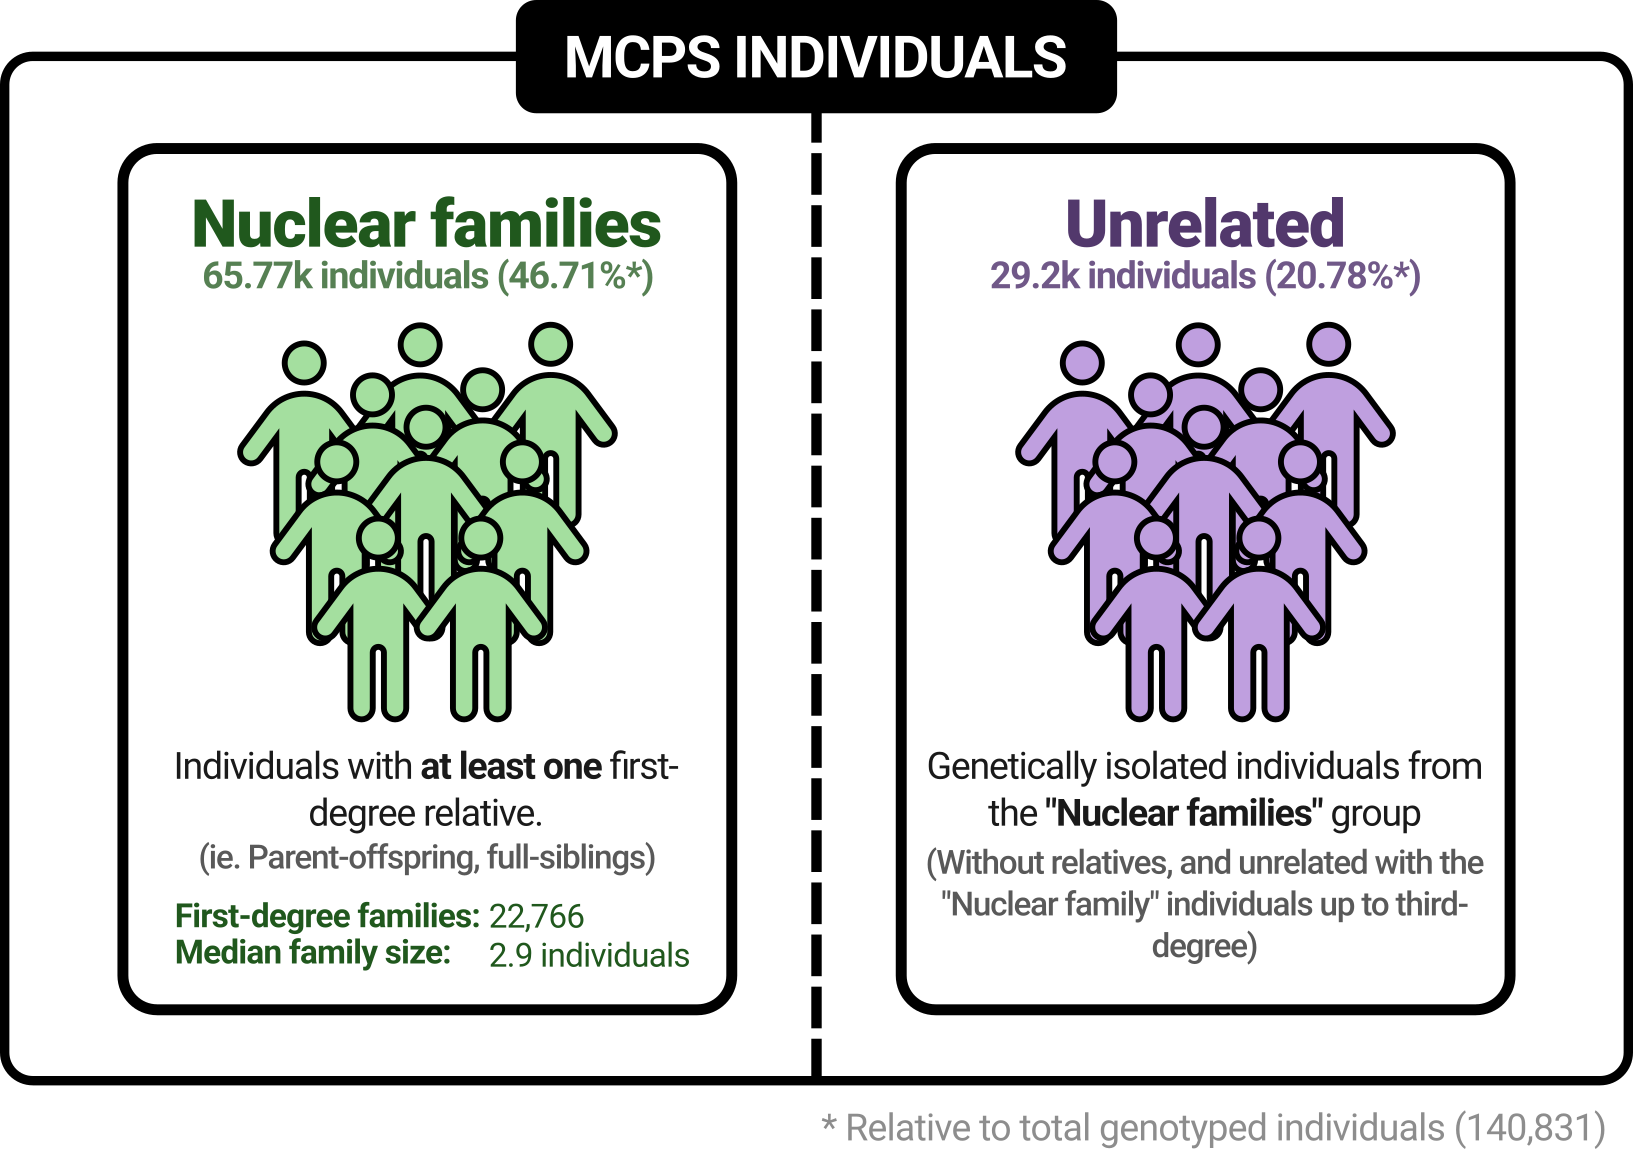
\includegraphics[width=0.90\textwidth]{img/diagrams/unrelated-individuals.png}
%     \end{column}
%   \end{columns}
% \end{frame}
% % \section{Results}
\section{Resultados}

% --- EFFECTIVE SAMPLE SIZE ---
\begin{frame}[c]{Tamaños Efectivos de Muestra}
  \begin{columns}[b]
    % --- LEFT COLUMN ----
    \begin{column}{0.64\textwidth}
      \centering
      
\includegraphics[width=\linewidth]{img/results/2026-02/effective-sample-sizes_robust-estimator_sibpair-trios.png}
    \end{column}
    % --- RIGHT COLUMN ----
    \begin{column}{0.36\textwidth}
      % --- UPPER QUADRANT ----
      \small\sffamily

      El estimador robusto tiene un mayor poder estadístico
      que el modelo de \textcite{young2022-fgwas}

      % --- LOWER QUADRANT ----
      \vspace{1cm}
      \vfill
      \captionof{figure}{
        \textbf{Comparación de tamaños efectivos de muestra para todos los rasgos en dos estimadores de FGWAS.}
        El estimador robusto vs. de pares de hermanos y trios parentales,
        incremento de 36.58\% (SD $\pm$ 6.78\%).
        Barras de error representan intervalos de confianza del 95\%.
      }
    \end{column}
  \end{columns}
\end{frame}

% --- HERITABILITY ---
\begin{frame}[c]{Estimaciones de heredabilidad}
  \begin{columns}[b]
    % --- Columna izquierda (imagen) ---
    \begin{column}{0.64\textwidth}
      \centering
      
\includegraphics[width=0.85\textwidth]{img/results/2026-02/heritability_comparison.scatter.png}
    \end{column}
    % --- Columna derecha (tabla + descripción) ---
    \begin{column}{0.36\textwidth}
      % Tabla escalada a 3 cm de altura (sin entorno table, innecesario en Beamer)
      \resizebox{0.99\textwidth}{!}{%
        \centering
        \small
        \begin{tabular}{llccrl}
          \toprule
          Trait type & Description & $h^2_{\mathrm{pop}}$ (SE) & $h^2_{\mathrm{DGE}}$ (SE) & $Z_{\mathrm{diff}}$ \\
          \midrule
          \multirow{6}{*}{Behavioural}
          & Current smoking vs former & 0.0132 (0.032) & 0.0005 (0.044) & -0.2336 \\
          & Current smoking vs not & 0.0144 (0.017) & 0.0148 (0.026) & 0.0129 \\
          & Educational attainment & 0.0721 (0.025) & 0.0106 (0.017) & -2.0510 \\
          & Frequency of alcohol consumption & 0.0244 (0.014) & 0.021 (0.028) & -0.1100 \\
          & Frequency of smoking & 0.0074 (0.019) & 0.0049 (0.027) & -0.0760 \\
          \multirow{8}{*}{Biomedical}
          & BMI & 0.1935 (0.021) & 0.1828 (0.029) & -0.2985 \\
          & DBP & 0.0913 (0.018) & 0.0942 (0.026) & 0.0923 \\
          & HDL cholesterol & 0.0893 (0.023) & 0.1455 (0.041) & 1.1895 \\
          & Height & 0.3312 (0.034) & 0.2247 (0.032) & -2.2604 \\
          & Hypertension & 0.0919 (0.019) & 0.0633 (0.024) & -0.9340 \\
          & LDL cholesterol & 0.146 (0.027) & 0.1113 (0.033) & -0.8088 \\
          & SBP & 0.1199 (0.022) & 0.1096 (0.029) & -0.2847 \\
          & Self-reported diabetes & 0.0903 (0.022) & 0.137 (0.03) & 1.2690 \\
          \bottomrule
        \end{tabular}
      }\par
      \vspace{1cm}
      \vfill
      \captionof{figure}{%
        \textbf{Comparación de estimaciones de heredabilidad derivadas de FGWAS contra PopGWAS.}
        Cada punto representa un rasgo complejo.
        Los colores representan la clasificación.
        La línea punteada representa la línea de identidad.
        Barras de error representan intervalos de confianza al 95\%.
      }
    \end{column}
  \end{columns}
\end{frame}

\begin{frame}[c]{Estimaciones de heredabilidad}
  \begin{columns}[b]
    % --- Columna izquierda (imagen) ---
    \begin{column}{0.64\textwidth}
      \centering
      
\includegraphics[width=0.85\textwidth]{img/results/2026-02/heritability_comparison.normalized.png}
    \end{column}
    % --- Columna derecha (tabla + descripción) ---
    \begin{column}{0.36\textwidth}
      % Tabla escalada a 3 cm de altura (sin entorno table, innecesario en Beamer)
      \resizebox{0.99\textwidth}{!}{%
        \centering
        \small
        \begin{tabular}{llccrl}
          \toprule
          Trait type & Description & $h^2_{\mathrm{pop}}$ (SE) & $h^2_{\mathrm{DGE}}$ (SE) & $Z_{\mathrm{diff}}$ \\
          \midrule
          \multirow{6}{*}{Behavioural}
          & Current smoking vs former & 0.0132 (0.032) & 0.0005 (0.044) & -0.2336 \\
          & Current smoking vs not & 0.0144 (0.017) & 0.0148 (0.026) & 0.0129 \\
          & Educational attainment & 0.0721 (0.025) & 0.0106 (0.017) & -2.0510 \\
          & Frequency of alcohol consumption & 0.0244 (0.014) & 0.021 (0.028) & -0.1100 \\
          & Frequency of smoking & 0.0074 (0.019) & 0.0049 (0.027) & -0.0760 \\
          \multirow{8}{*}{Biomedical}
          & BMI & 0.1935 (0.021) & 0.1828 (0.029) & -0.2985 \\
          & DBP & 0.0913 (0.018) & 0.0942 (0.026) & 0.0923 \\
          & HDL cholesterol & 0.0893 (0.023) & 0.1455 (0.041) & 1.1895 \\
          & Height & 0.3312 (0.034) & 0.2247 (0.032) & -2.2604 \\
          & Hypertension & 0.0919 (0.019) & 0.0633 (0.024) & -0.9340 \\
          & LDL cholesterol & 0.146 (0.027) & 0.1113 (0.033) & -0.8088 \\
          & SBP & 0.1199 (0.022) & 0.1096 (0.029) & -0.2847 \\
          & Self-reported diabetes & 0.0903 (0.022) & 0.137 (0.03) & 1.2690 \\
          \bottomrule
        \end{tabular}
      }\par
      \vspace{0.15cm}
      {\centering
        \begin{equation*}
            Z_{\mathrm{diff}} = \frac{
                \Delta h^2_{\mathrm{pop - DGE}}
            }{
                \sqrt{SE^2_{\mathrm{pop}} - SE^2_{\mathrm{DGE}}}
            }
        \end{equation*}
      }\par
      \vspace{0.15cm}
      \vfill
      \captionof{figure}{%
        \textbf{Diferencias normalizadas entre estimaciones de heredabilidad.}
        La diferencia asume independencia entre las muestras del FGWAS y popGWAS,
        y son respecto a las estimaciones de popGWAS.
      }
    \end{column}
  \end{columns}
\end{frame}

% --- EFFECT SIZE CORRELATIONS ---
\begin{frame}[c]{Correlación de estimadores}
\begin{figure}
    \begin{minipage}[b]{0.67\textwidth}
        
\includegraphics[width=0.95\textwidth]{img/results/2026-02/snipar-correlations.png}
    \end{minipage}\hfill
    \begin{minipage}[b]{0.33\textwidth}
        \caption{
            \textbf{Correlaciones de genoma completo entre efectos genéticos directos y efectos poblacionales.}
            Correlaciones estimadas con snipar \parencite{young2022-fgwas}
            entre efectos genéticos directos y poblacionales,
            ajustado para LD y correlaciones muestrales.
            Comparaciones contrastadas con resultados de \textcite{tan2024-fgwas}.
            Barras de error indican intervalos de confianza al 95\%.
        }
    \end{minipage}
\end{figure}
\end{frame}

% \section{Conclusiones}

\begin{frame}[c]{Conclusiones}
    \begin{enumerate}
        \item \textbf{El estimador robusto de snipar incrementa el tamaño de muestra efectivo} respecto al método de \textcite{young2022-fgwas}, mejorando la precisión de las estimaciones de heredabilidad en el diseño familiar.
        \item \textbf{Las heredabilidades estimadas en el diseño familiar tienden a ser menores} que en el poblacional. Tres rasgos biomédicos ---diabetes reportada, colesterol HDL y presión arterial diastólica--- muestran el patrón opuesto.
        \item \textbf{El poder estadístico en MCPS es limitado para detectar correlaciones} entre efectos poblacionales ($\hat{\beta}$) y familiares ($\hat{\delta}$), particularmente en rasgos con baja heredabilidad.
        % Esto implica que las correlaciones observadas deben interpretarse a la luz de simulaciones de poder, y no necesariamente como evidencia de ausencia de concordancia entre diseños.
    \end{enumerate}
\end{frame}

\begin{frame}[c]{Perspectivas y trabajo futuro}
    \begin{itemize}
        \item \textbf{Comprobar diferencias de heredabilidad} con pruebas estadísticas apropiadas
        \item \textbf{Complementar comparaciones} con pruebas de heterogeneidad DGEs vs. efectos poblacionales en SNPs indpendientes (\textit{clumping} de $r^2 < 1\%$), con FDR a 5\% y 10\%.
        \item (Opcional) \textbf{Diagnosticar el estimador (correlaciones)} de \textcite{young2022-fgwas}, ¿Cuál es la razón por la que los rasgos de MCPS parece tener bajo poder?
        \item (Opcional) Proceder a fine-mapping.
    \end{itemize}
\end{frame}

% Tutors
% ============================================================
% Tutors Slide
% ============================================================
\begin{frame}{Current collaborations}

  \vfill

  % --- Row 1 ---
  \centering
  \tutorcard{img/tutors/jason-torres.png}{0.8cm}
    {PhD. Jason Torres}
    {Senior Genetics Epidemiologist}
    {CTSU, NDPH -- University of Oxford}
  \hfill
  \tutorcard{img/tutors/mashaal-sohail.jpeg}{0.8cm}
    {PhD. Mashaal Sohail}
    {Main PhD Supervisor}
    {CCG -- UNAM}
  \hfill
  \tutorcard{img/tutors/alexander-young.jpeg}{0.8cm}
    {PhD. Alexander S. Young}
    {Mendelian Imputation author}
    {Human Genetics Dept. -- UCLA}
  \vfill

  % --- Row 2 ---
  \tutorcard{img/tutors/daniela-robles-espinoza.jpg}{0.8cm}
    {PhD. Carla D. Robles Espinoza}
    {Member of Tutor Committee}
    {LIIGH -- UNAM}
  \hspace{2.5em}
  \tutorcard{img/tutors/jaime-berumen.png}{0.8cm}
    {PhD. Jaime Berumen Campos}
    {Member of Tutor Committee}
    {MCPS P.I. | UIME -- UNAM}
\end{frame}

\begin{frame}[plain]{}

  \centering

  % --- Logos row ---
  
\includegraphics[height=0.7cm]{img/logos/unam-logo.png}%
  \hfill
  
\includegraphics[height=0.7cm]{img/logos/ccg-logo.png}%
  \hfill
  
\includegraphics[height=0.7cm]{img/logos/pdcb.png}%
  \hfill
  
\includegraphics[height=0.7cm]{img/logos/oxford-ctsu.png}%
  \hfill
  
\includegraphics[height=0.7cm]{img/logos/mcps.png}%

  \vfill

  {\Large\bfseries\color{ccgblue} ¡GRACIAS A TODXS!}

  \vfill

  \begin{minipage}[t]{0.45\textwidth}
    \centering
    \begin{tikzpicture}
      \node[inner sep=0pt, rounded corners=4pt, clip]
        {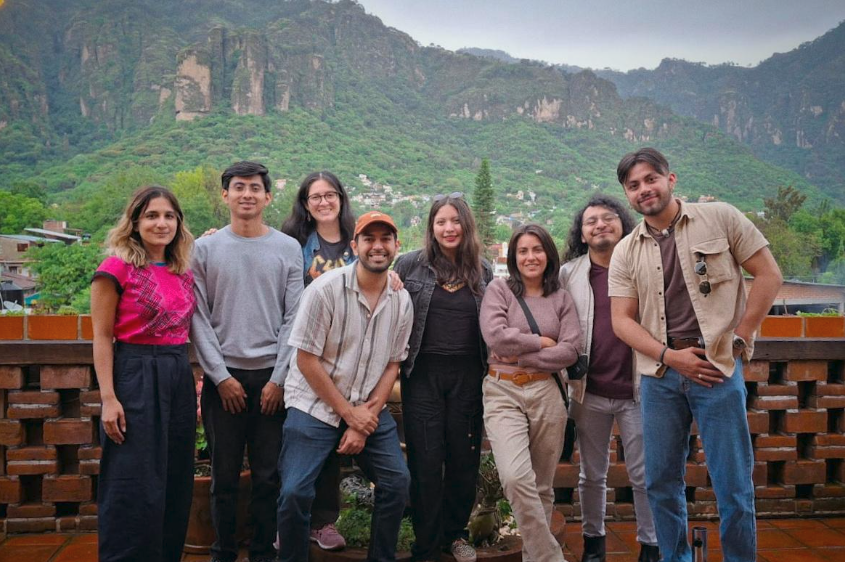
\includegraphics[width=\textwidth, height=4cm, keepaspectratio]{img/tutors/sohail-lab.png}};
    \end{tikzpicture}\\[4pt]
    {\sffamily\color{ccgblue!50!black}%
      {\scriptsize\bfseries Sohail Lab}\\[-2pt]
      {\tiny Centro de Ciencias Genómicas (CCG)}\\[-5pt]
      {\tiny Universidad Nacional Autónoma de México (UNAM)}\\[-5pt]
      {\tiny Cuernavaca, Morelos, MX.}
    }
  \end{minipage}
  \hfill
  \begin{minipage}[t]{0.45\textwidth}
    \centering
    \begin{tikzpicture}
      \node[inner sep=0pt, rounded corners=4pt, clip]
        {
\includegraphics[width=\textwidth, height=4cm, keepaspectratio]{img/tutors/oxford-team.png}};
    \end{tikzpicture}\\[4pt]
    {\sffamily\color{ccgblue!50!black}%
      {\scriptsize\bfseries Mexico City Prospective Study (MCPS) team}\\[-2pt]
      {\tiny Clinical Trial Service Unit (CTSU)}\\[-5pt]
      {\tiny University of Oxford}\\[-5pt]
      {\tiny Oxford, Oxfordshire, U.K.}
    }
  \end{minipage}

\end{frame}

% Bibliography ----
% \begin{frame}
%     \frametitle{References}
%     \begin{multicols}{2}
%         \printbibliography[]
%     \end{multicols}
% \end{frame}

\end{document}
